\documentclass[UTF8,11pt]{ctexart}
\usepackage[a4paper,margin=2.3cm]{geometry}
\usepackage{amsmath,amssymb,amsthm}
\usepackage{booktabs}
\usepackage{graphicx}
\usepackage{float}
\usepackage[numbers]{natbib}
\usepackage{hyperref}
\usepackage{xcolor}
\usepackage{enumitem}
\usepackage{array}
\usepackage{longtable}
\usepackage{caption}
\graphicspath{{figures/}{./}}
\hypersetup{colorlinks=true,linkcolor=blue,citecolor=blue,urlcolor=blue}
\captionsetup{font=small}
\newcounter{algobox}
\renewcommand{\thealgobox}{\arabic{algobox}}
\newcommand{\algcaption}[1]{\refstepcounter{algobox}\caption*{\textbf{算法\thealgobox：}#1}}

\newtheorem{proposition}{命题}
\newtheorem{remark}{评注}
\newtheorem{assumption}{假设}
\newcommand{\qos}{q}
\newcommand{\T}{\mathcal{T}}
\newcommand{\J}{\mathcal{J}}
\newcommand{\N}{\mathcal{N}}
\newcommand{\A}{\mathcal{A}}
\newcommand{\D}{D}
\newcommand{\U}{U}
\newcommand{\w}{\boldsymbol{w}}
\newcommand{\p}{\boldsymbol{p}}
\newcommand{\g}{\boldsymbol{g}}

\title{\textbf{面向Token推理服务的三方跨时段定价博弈：\\
平台--中间商--用户结构下的批发价格、容量分配与QoS反馈}}
\author{匿名作者}
\date{\today}

\begin{document}
\maketitle

\begin{abstract}
大模型推理服务具有明显的时段性负载波动。峰时请求会推高首token延迟、超时率和SLA违约风险，进而降低可结算服务量。本文研究一个单平台、多中间商和用户共同参与的三层推理服务市场：平台发布分时批发价，中间商非合作地选择零售价与跨时段容量分配，用户依据价格、时段偏好、原生时段分布、迁移成本和预期QoS选择中间商--时段组合；扩展实验进一步允许用户选择厂家直供API作为平台自营通道。理论上，本文在用户层构造有限拥塞博弈并证明纯策略Nash均衡存在，推导logit随机用户均衡与QoS固定点，给出中层凹博弈条件下的均衡存在性和三层Stackelberg子博弈完美均衡的充分条件。数值上，本文只将求解结果解释为采样批发价集合和SLSQP最优响应范围内的solver-based regret候选均衡，不作为非凸问题的全局Nash证书。合成基准下，三层QoS感知策略相对统一零售基线将最低QoS从0.8428提高到1.0000，系统利润从4911.97提高到9525.12；相对忽略QoS的动态策略，系统利润提高13.61\%。补充实验从机制归因、鲁棒性、用户福利、价格保护、厂家直供API、校准压力和vLLM测量QoS等方面检验适用边界。结果表明，无约束收入最大化仍会降低用户侧inclusive value；在价格保护、足够直供容量和受控价格区间下，平台收入目标可以与更高的用户侧inclusive value和QoS同时成立。本文方法的现实定位是离线机制仿真和策略筛选工具，生产部署仍需要真实请求轨迹、用户弹性和合约约束校准。
\end{abstract}

\noindent\textbf{关键词：}推理服务；Token定价；中间商；Stackelberg博弈；拥塞博弈；Nash均衡；跨时段容量分配；QoS反馈

% ============================================================
\section*{术语表}
\label{sec:nomenclature}

\begin{longtable}{@{}p{0.28\textwidth}p{0.68\textwidth}@{}}
\toprule
符号 & 含义 \\
\midrule
\endhead
\multicolumn{2}{l}{\textbf{集合与索引}} \\
$\T=\{1,\ldots,T\}$ & 时段集合 \\
$\J=\{1,\ldots,J\}$ & 中间商集合 \\
$\N=\{1,\ldots,N\}$ & 用户集合 \\
$\A=\J\times\T$ & 用户可选中间商--时段组合集合 \\
$\A^+=(\J\cup\{0\})\times\T$ & 含厂家直供API通道的扩展用户选择集合 \\
\midrule
\multicolumn{2}{l}{\textbf{变量}} \\
$w_t$ & 平台在时段$t$的批发价格 \\
$p_{j,t}$ & 中间商$j$在时段$t$的零售价格 \\
$g_{j,t}$ & 中间商$j$在时段$t$分配的可服务容量 \\
$\D_{j,t}$ & 流向中间商$j$时段$t$的总需求 \\
$q_{j,t}=\qos(\cdot)$ & 中间商$j$时段$t$的QoS（有效完成服务比例） \\
$p^D_t,g^D_t,\D^D_t,q^D_t$ & 厂家直供API通道在时段$t$的零售价、容量、需求和QoS \\
$u_{j,t}$ & 中间商$j$时段$t$的局部利用率 \\
$s_{j,t}$ & 用户选择中间商$j$时段$t$的logit份额 \\
$\Pi^P$ & 平台批发收入 \\
$\Pi^{P,+}$ & 含厂家直供API净收益的平台收益 \\
$\Pi^I$ & 中间商总利润 \\
$\Pi^S$ & 系统总利润 \\
\midrule
\multicolumn{2}{l}{\textbf{参数}} \\
$h$ & 每时段时长（小时） \\
$G_j$ & 中间商$j$的总容量预算 \\
$\bar u$ & QoS退化阈值利用率 \\
$\kappa$ & QoS退化强度 \\
$\alpha$ & 用户价格敏感度 \\
$c_s$ & 用户跨时段迁移成本 \\
$c_g$ & 单位容量成本 \\
$c_q$ & 单位QoS退化成本 \\
$\bar F$ & 基础需求规模 \\
$a_t$ & 时段$t$的用户偏好因子 \\
$\pi_t$ & 用户原生偏好时段分布，$\sum_t\pi_t=1$ \\
$b_j$ & 中间商$j$的品牌/便利性因子 \\
$p_0$ & 基准零售价 \\
$\underline g$ & 数值容量正下界 \\
\bottomrule
\caption{模型符号表}
\label{tab:nomenclature}
\end{longtable}

% ============================================================
\section{引言}

\subsection{研究背景}

大模型推理服务已经从离线批处理逐步转向持续运行的在线服务。交互式聊天、代码生成、自动代理、离线评测和周期性工作流在一天内呈现不同的到达规律，使GPU推理集群面临显著的峰谷差。系统研究表明，批处理、资源共享、内存管理和请求调度会同时影响吞吐、延迟和成本\cite{crankshaw2017clipper,gujarati2020clockwork,romero2021infaas,yu2022orca,kwon2023pagedattention,agrawal2024sarathiserve}。当利用率接近容量边界时，首token延迟、排队时间和有效完成率会快速变化，服务质量的退化将直接影响可结算服务量和用户满意度。

在推理服务市场中，上游平台（如拥有GPU集群的模型厂家或API提供商）需要协调下游中间商（代理平台、行业服务商、API聚合器）和终端用户之间的资源分配。然而，现实中平台并不直接面向所有终端用户出一零售价，中间商作为独立利益主体，会根据批发价格自主选择跨时段的零售定价和容量分配策略。例如，OpenRouter类API聚合商管理的token预算和模型路由决定了其向终端用户提供的服务组合。中间商的容量分配和零售价格又会直接影响用户在不同时段和中间商之间的迁移选择，进而改变局部拥塞状态和QoS表现。因此，面对包含多个利益主体的复杂系统优化问题，平台需要为中间商制定内部分时批发价。现实部署中的批发定价通常不能只追求平台短期收入最大化，还需要观察下游利润、用户体验和SLA约束；本文先研究平台收入作为领导者目标时的价格传导，并在实验中单独报告系统利润、QoS和用户福利诊断。

在此背景下，一个关键研究问题随之浮现：在推理服务存在时段性负载波动和QoS退化的情况下，平台应如何制定分时批发价格，使其在中间商自主优化和用户自由迁移的条件下，形成稳定的下游响应、提升系统利润并改善QoS底线？该问题不能由单层利润最大化直接描述，因为用户需求不是外生常数、中间商并非被动转发价格、QoS也不是固定参数，而是由需求和容量共同决定的内生变量。解决这一问题，是推理服务跨时段协调定价研究的重要方向。

\subsection{文献综述与研究缺口}
\label{sec:related_work}

现有文献中，推理服务的定价问题通常与系统调度或资源管理策略结合研究\cite{crankshaw2017clipper,yu2022orca,kwon2023pagedattention}。这些研究大多聚焦于两个方面：给定请求集下如何通过批处理、缓存和调度提高执行效率，以及不同模型或GPU云之间的性价比比较。其中，Clipper、Clockwork和INFaaS展示了机器学习服务中模型选择、调度和资源管理的重要性\cite{crankshaw2017clipper,gujarati2020clockwork,romero2021infaas}。Orca、PagedAttention、Sarathi-Serve、Splitwise、DistServe和Vidur等工作进一步针对大模型推理中的批处理、KV缓存、prefill-decode干扰和模拟器规划提出系统优化方法\cite{yu2022orca,kwon2023pagedattention,agrawal2024sarathiserve,patel2024splitwise,zhong2024distserve,agrawal2024vidur}。但这些研究解答的是给定请求集合如何执行得更快，通常不把需求迁移、零售渠道和平台收益放入同一个博弈模型。

在定价和市场机制方面，近期研究已经开始把大模型推理服务视为同时具有技术成本和经济响应的市场系统，讨论推理成本、菜单定价、Stackelberg定价/路由以及位置化价格等问题\cite{demirer2025emerging,erdil2025inference,bergemann2025menu,guo2026prillm,yan2026stackelberg,liu2026locational}。例如，Yan等提出Stackelberg博弈，把LLM推理服务提供商和客户之间的批处理偏好和延迟成本纳入价格--调度联合优化；Liu等的工作涉及地理分散推理集群的位置定价和多市场出清；菜单定价和token容量合约相关工作则表明，用户选择集合与合同结构会影响服务定价结果\cite{bergemann2025menu,xing2026tokenfutures}。这些工作说明，LLM推理定价已经不是单纯的系统吞吐优化问题，而是需要同时考虑成本、需求响应、服务质量和策略互动。

本文将研究缺口限定为一个更具体的组合问题：在同一个可计算模型中，同时保留战略中间商、跨时段容量分配、用户迁移和内生QoS反馈。现有工作通常重点处理其中一部分，例如系统调度、平台--用户直接定价、批处理偏好、地理市场出清或合同菜单；在代理平台、API聚合器和企业转售商参与的场景中，中间商还会自主决定零售价、模型路由和容量预算。若把中间商简化为被动加价渠道，就难以刻画批发价格→零售价格→用户迁移→局部拥塞→QoS反馈→有效结算量这一价格传导链。本文因此把中间商作为具有独立策略空间的博弈主体，并把用户选择和QoS退化嵌入同一三层响应系统。

除利益主体的博弈建模之外，推理服务定价研究中另一个关键方法论考量是QoS退化的不确定性处理。拥塞定价和收益管理文献提供了价格协调有限容量和异质需求的理论基础\cite{vickrey1969congestion,gallego1994dynamic,elmaghraby2003dynamic,bitran2003overview,talluri2004revenue,phillips2005pricing}。电力市场中的实时定价和需求响应研究提供了跨时段负载迁移的机制类比\cite{schweppe1988spot,borenstein2005long,albadi2008summary,faruqui2010household,siano2014demand}。对于本文模型中的QoS退化函数，延迟、完成率、吞吐和SLA达标率是推理请求的核心服务质量指标。不同于电力出清依赖潮流方程，推理服务的QoS退化取决于局部利用率和请求到达过程。本文的建模将拥塞博弈、随机效用离散选择模型和logit均衡结合，以有限参与者博弈到连续需求响应的极限过渡为理论基础\cite{rosenthal1973class,monderer1996potential,wardrop1952some,sandholm2010population,mcfadden1974conditional,train2009discrete}。将势博弈的PSNE存在性证明与可微logit SUE连接，并在三层Stackelberg博弈中通过逆向归纳定义均衡，为推理服务跨时段定价提供了一个具有明确理论边界且可计算的博弈论框架。

\subsection{贡献与文章组织}

为弥补上述研究缺口，本文研究一个单平台、多中间商和异质用户共同参与的Token推理服务三层市场，在考虑多利益主体博弈关系和中间商策略自由度的同时，纳入QoS退化反馈链。本文的主要贡献如下。

\begin{enumerate}[leftmargin=2em]
  \item \textbf{QoS反馈下的三层Stackelberg博弈框架：} 不同于现有研究将中间商视为被动转发渠道或将QoS视为固定参数，本文模型建立了批发价格→中间商零售价与容量分配→用户迁移→局部拥塞→QoS反馈→利润的反馈链。在此框架中，平台的批发定价通过影响中间商的利润空间而改变其零售价和容量分配策略，中间商的决策通过用户logit选择改变各时段的需求分布和局部利用率，QoS退化反过来影响有效结算量和中间商利润。这为理解推理服务中批发--零售渠道的价格传导机制和QoS退化成本的内化过程提供了新视角。
  \item \textbf{三层博弈模型、条件性均衡存在证明与regret-bounded数值候选：} 用户层构造有限拥塞博弈和Rosenthal势函数，证明纯策略Nash均衡（PSNE）存在；从随机效用模型推导logit随机用户均衡（SUE），并解释有限参与者均衡到大人口logit响应的理论联系。中间商层写出包含零售收入、批发成本、容量成本和QoS退化成本的利润函数，推导一阶条件和容量约束KKT条件。平台层通过逆向归纳定义子博弈完美均衡（SPE），并在标准正规条件下给出条件性存在证明。为支撑数值实现，本文进一步给出用户层连续固定点、中层凹博弈存在性条件和solver-based regret诊断。这一从微观到宏观、从离散到连续的推导，为推理服务的多层市场设计提供了可复核的理论边界。
  \item \textbf{可复现的数值实验与多基线对比：} 合成基准下实现五类策略对比（统一零售、平台直销、单中间商、无QoS动态定价、三层QoS感知定价），并系统报告平台批发收入、中间商利润、系统利润、最低QoS、峰值利用率和中间商solver-based regret。为避免把单一合成场景外推为生产结论，本文把补充实验分为四组：机制归因与有限用户桥接、算法与参数鲁棒性、vLLM测量QoS和测量驱动到达率重放、用户保护与厂家直供API outside option。实验结果和图表均由可复现代码直接生成，并用于界定收入、QoS和用户体验改善同时成立的条件区域。
\end{enumerate}

本文余下结构与三层博弈建模顺序对应。第~\ref{sec:problem} 节给出问题描述和多利益主体信息交互关系。第~\ref{sec:formulation} 节给出上层平台、中层中间商和下层用户的数学模型及三层Stackelberg博弈定义。第~\ref{sec:solution} 节描述均衡求解的固定点视角和迭代分布式算法。第~\ref{sec:case_study} 节报告案例研究结果与讨论。第~\ref{sec:conclusion} 节总结全文。

% ============================================================
\section{问题描述}
\label{sec:problem}

在一个推理服务市场中，多个自主主体参与token交易并具有相互依赖但存在冲突的经济利益。本文将这些主体称为利益相关方。具体而言，如图~\ref{fig:three_layer_framework} 所示，考虑一个拥有或租用上游GPU推理能力的单一平台，该平台聚合了三类下游利益主体：多个中间商（代理平台、行业应用服务商、API聚合器或转售商）以及终端用户。中间商位于平台和用户之间，从平台购买推理能力，将其重新包装后销售给终端用户；用户具有不同的时段偏好、迁移成本和价格敏感度，可以在多个中间商和多个时段之间选择。平台与中间商通过批发价进行token交易，中间商与用户通过零售价进行服务交易。假设平台、中间商和用户分属不同的利益主体，各自独立决策。

该多利益主体设定天然产生利益冲突。平台倾向于提高批发价以增加上游收入，但过高的批发价会压缩中间商利润空间，导致零售价上升和需求流失。中间商希望提高零售价和容量利用率以获取更高毛利，但过度追求短期利润会造成局部拥塞，降低QoS并减少有效结算量，进而反向损害自身利润。用户希望选择价格低、偏好匹配且QoS高的中间商--时段组合，但个体选择聚集到同一时段后会改变拥塞状态，反过来影响所有选择该组合的用户。平台批发价影响中间商利润空间，中间商零售价和容量影响用户迁移，用户迁移改变局部拥塞，QoS改变有效服务量和利润，再反向影响上层定价。这些相互关联的决策构成一个复杂的分层互动，无法用单层优化模型描述。

因此，关键研究挑战在于确定：平台应如何设计分时批发价格和中间商调度策略，使得当所有利益相关方追求各自的个体目标时，最终结果达到一个没有参与者能够单方面改善自身地位的均衡。这样的均衡可为利益相关方之间的推理服务交互提供稳定的价格--容量响应关系，但其福利含义仍取决于平台目标函数和额外参与约束。

为解决这一挑战，本文提出一个三层Stackelberg博弈框架，显式建模利益相关方之间的分层决策结构。如图~\ref{fig:three_layer_framework} 所示，上层平台抽象展开为DeepSeek、Claude、GPT/OpenAI等模型厂家和上游API供给网络；中层中间商画成OpenRouter类API聚合商、企业转售商和应用平台。平台作为上层领导者，发布分时批发价$\w$；中间商作为中层追随者（同时也是下层用户群的领导者），观察批发价后同时选择零售价$\p$和跨时段容量分配$\g$；用户作为下层追随者，观察零售价和预期QoS后选择中间商--时段组合$(j,t)$。该三层博弈的均衡解提供了协调推理服务中批发定价、零售定价和容量分配的计算方案。

\begin{figure}[H]
\centering
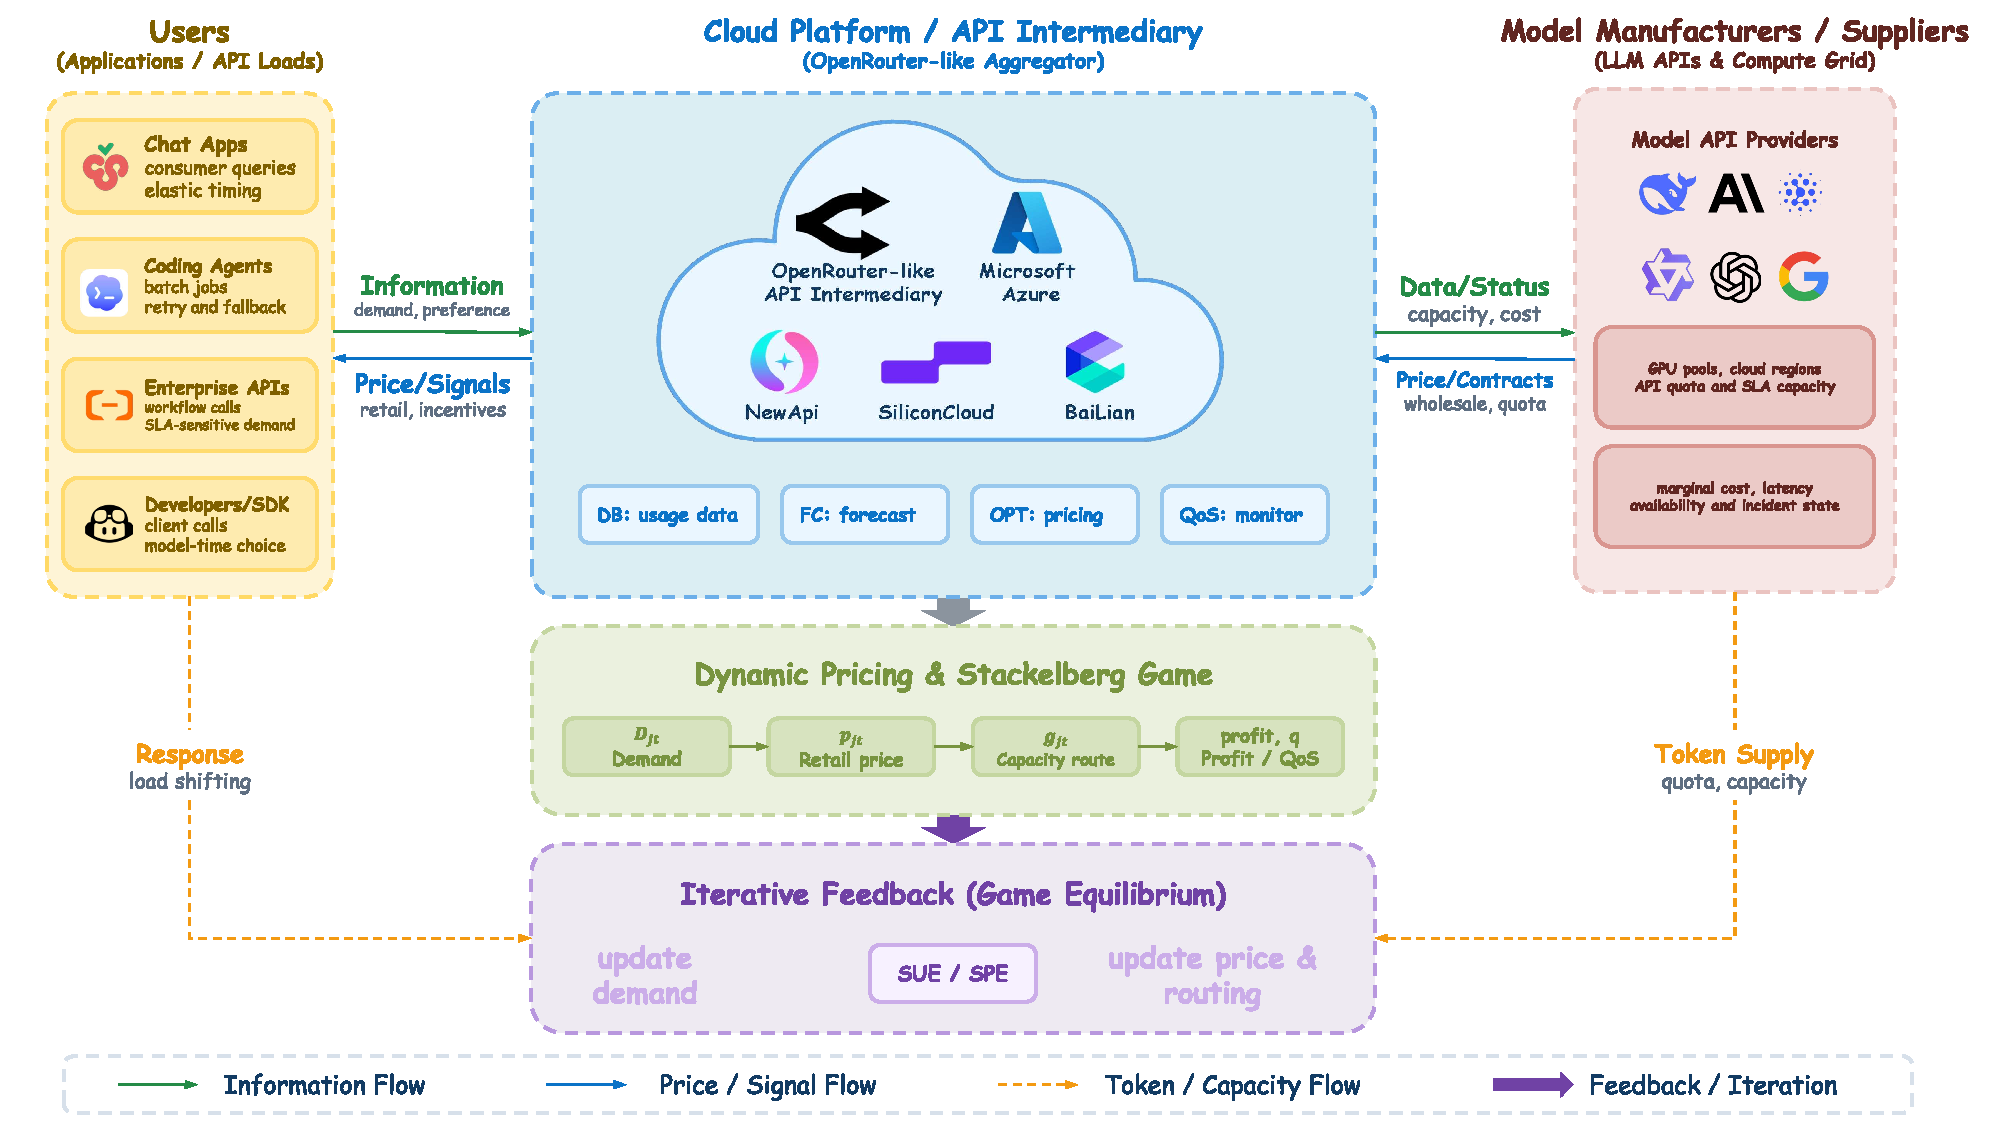
\includegraphics[width=\textwidth]{figures/three_layer_game_framework.pdf}
\caption{模型厂家--API中间商--应用/用户的互联三层博弈图。上游模型厂家包括DeepSeek、Claude、GPT/OpenAI等API供给方；OpenRouter类聚合商和企业转售商选择模型路由、容量和零售价；用户在中间商--时段组合$(j,t)$间迁移，中间商再把需求路由到上游模型API。需求形成局部利用率，QoS再反向影响可结算服务量、利润和价格更新。}
\label{fig:three_layer_framework}
\end{figure}

% ============================================================
\section{数学模型}
\label{sec:formulation}

设一天被划分为$T$个时段$\T=\{1,\ldots,T\}$，中间商集合为$\J=\{1,\ldots,J\}$，用户集合为$\N=\{1,\ldots,N\}$。平台发布批发价向量$\w=(w_1,\ldots,w_T)$。中间商$j$为时段$t$分配可服务容量$g_{j,t}\ge \underline g>0$，并发布零售价$p_{j,t}$。用户选择一个中间商--时段组合$(j,t)$。服务质量由中间商局部负载决定：
\begin{equation}
  u_{j,t}=\frac{\D_{j,t}}{g_{j,t}},\qquad
  q_{j,t}=\qos(u_{j,t})=
  \begin{cases}
    1, & u_{j,t}\le \bar u,\\
    \exp[-\kappa(u_{j,t}-\bar u)^2], & u_{j,t}>\bar u.
  \end{cases}
  \label{eq:qos}
\end{equation}
其中$\D_{j,t}$是流向中间商$j$在时段$t$的总需求。若$g_{j,t}$过小或$\D_{j,t}$过大，则$q_{j,t}$下降，表示有效完成服务比例下降。

平台收入、中间商利润和系统利润分别为
\begin{align}
  \Pi^P(\w,\p,\g)
  &=h\sum_{j\in\J}\sum_{t\in\T} w_t\D_{j,t}q_{j,t}, \label{eq:platform_profit}\\
  \Pi^I(\w,\p,\g)
  &=h\sum_{j,t}(p_{j,t}-w_t)\D_{j,t}q_{j,t}
    -h\sum_{j,t}c_g g_{j,t}
    -h\sum_{j,t}c_q(1-q_{j,t})\D_{j,t}, \label{eq:intermediary_profit}\\
  \Pi^S(\w,\p,\g)&=\Pi^P+\Pi^I. \label{eq:system_profit}
\end{align}
该定义把平台批发收入与中间商零售毛利分开报告。QoS下降既减少有效结算量，也通过$c_q$表示SLA违约、用户流失或服务补偿成本。

在用户可同时选择厂家直供API的扩展场景中，用户行动集合变为
\begin{equation}
  \A^+=(\J\cup\{0\})\times\T,
  \label{eq:direct_api_action_set}
\end{equation}
其中$j=0$表示平台自营的厂家直供API通道。该通道具有直供零售价$p^D_t$和直供容量$g^D_t$，与中间商通道共同进入用户logit选择。此时平台收益可写为
\begin{equation}
  \Pi^{P,+}
  =h\sum_{j\in\J}\sum_{t\in\T}w_t\D_{j,t}q_{j,t}
  +h\sum_{t\in\T}\left[
    p^D_t\D^D_tq^D_t-c_g g^D_t-c_q(1-q^D_t)\D^D_t
  \right],
  \label{eq:direct_platform_payoff}
\end{equation}
其中第一项是平台从中间商获得的批发收入，第二项是厂家直供API的净收益。中间商利润仍只在$j\in\J$上计算。本文把该扩展作为补充实验，用于检验直供API作为用户outside option时是否会约束中间商定价，以及如何影响用户体验。
在该扩展中，式~\eqref{eq:logit_share} 的归一化范围和式~\eqref{eq:demand} 中的份额求和相应扩展到$\J\cup\{0\}$。数值实验先固定$p^D_t$和$g^D_t$检验直供通道作为外部选项的约束作用，再通过价格--容量扫描检验该约束作用的参数边界；本文不把该扩展解释为直供价格--容量联合最优设计。

\subsection{上层模型：平台批发定价}
\label{sec:upper_platform}

平台在上层选择$\w\in[\underline w,\overline w]^T$。平台不直接控制下层需求，而是预期中间商和用户响应后形成的有效服务量$\D_{j,t}q_{j,t}$。平台问题为
\begin{equation}
  \max_{\w\in[\underline w,\overline w]^T}\;
  \Pi^P(\w,\p^*(\w),\g^*(\w)),
  \label{eq:platform_problem}
\end{equation}
其中$(\p^*(\w),\g^*(\w))$表示中间商层的均衡响应，用户需求由下层选择模型给出。式~\eqref{eq:platform_problem} 对应三层博弈中的领导者问题：平台调节的是批发价格，而非终端零售价格和用户选择本身。

式~\eqref{eq:platform_problem} 刻画的是平台收入目标，而不是社会福利目标。若运营者希望把用户福利或下游参与约束显式放入上线决策，可在平台层加入
\begin{equation}
  \Pi^I_j(\w,x)\ge \Pi^{I,\mathrm{ref}}_j,\quad
  W^U(\p,\g)\ge W^{U,\mathrm{ref}},\quad
  \bar q_{\mathrm{active}}\ge q_{\mathrm{SLA}},
  \label{eq:deployment_constraints}
\end{equation}
其中$W^U(\p,\g)=\log\sum_{j,t}\exp(z_{j,t})$是logit模型对应的用户侧inclusive value，$\bar q_{\mathrm{active}}$表示活跃需求单元上的服务质量指标。本文主实验先采用平台收入最大化作为Stackelberg领导者问题，再在实验部分单独报告系统利润、中间商利润、QoS和平台候选参考搜索，用于识别平台目标与系统目标是否出现张力。

\subsection{中层模型：中间商零售定价与容量分配}
\label{sec:middle_intermediary}

给定平台批发价$\w$，中间商$j$观察上层价格后选择$\g_j=(g_{j,1},\ldots,g_{j,T})$和$\p_j=(p_{j,1},\ldots,p_{j,T})$，满足
\begin{equation}
  \sum_{t=1}^{T}g_{j,t}=G_j,\qquad g_{j,t}\ge \underline g,\qquad
  p_{j,t}\in[\underline p,\overline p].
  \label{eq:capacity_constraint}
\end{equation}
其中$\underline g$是避免$D/g$奇异的容量正下界，要求$G_j\ge T\underline g$。数值实现取$\underline g=10^{-6}$，相对于$G_j$的量级可忽略。
在其他中间商策略固定时，中间商$j$的最优响应为
\begin{equation}
  \mathcal{BR}_j(\w,x_{-j})=
  \arg\max_{x_j\in\Omega_j}\;
  \left[
  h\sum_{t}(p_{j,t}-w_t)\D_{j,t}q_{j,t}
  -h\sum_t c_g g_{j,t}
  -h\sum_t c_q(1-q_{j,t})\D_{j,t}
  \right],
  \label{eq:broker_problem}
\end{equation}
其中$x_j=(\p_j,\g_j)$，$x_{-j}$表示除$j$以外的其他中间商策略，$\Omega_j$由式~\eqref{eq:capacity_constraint}给出。给定$\w$，中层Nash响应$x^*$满足$x_j^*\in\mathcal{BR}_j(\w,x_{-j}^*)$对所有$j\in\J$成立。
该目标函数包含零售收入、批发成本、容量成本和QoS退化成本。与只优化价格的模型不同，中间商还必须决定跨时段容量如何分配。容量过少会提高利用率并降低QoS，容量过多则增加闲置成本。

\subsubsection{零售价一阶条件}

令$M_{j,t}=(p_{j,t}-w_t)q_{j,t}-c_q(1-q_{j,t})$为每单位需求的有效边际收益。忽略边界时，零售价的一阶条件为
\begin{equation}
  \frac{\partial\Pi^I_j}{\partial p_{j,t}}
  =h\left[
  \D_{j,t}q_{j,t}
  +M_{j,t}\frac{\partial \D_{j,t}}{\partial p_{j,t}}
  +(p_{j,t}-w_t+c_q)\D_{j,t}\frac{\partial q_{j,t}}{\partial p_{j,t}}
  \right]=0.
  \label{eq:retail_foc}
\end{equation}
第一项是提高零售价带来的直接收入，第二项是价格上升导致需求下降的损失，第三项是需求变化通过利用率改变QoS后的间接影响。

\subsubsection{容量分配KKT条件}

容量分配的拉格朗日函数为
\begin{equation}
  \mathcal{L}_j=\Pi^I_j+\lambda_j\left(G_j-\sum_t g_{j,t}\right)
  +\sum_t \mu_{j,t}(g_{j,t}-\underline g).
  \label{eq:broker_lagrangian}
\end{equation}
KKT条件为
\begin{align}
  \frac{\partial\Pi^I_j}{\partial g_{j,t}}-\lambda_j+\mu_{j,t}&=0,
  \label{eq:kkt_stationarity}\\
  \sum_t g_{j,t}=G_j,\quad g_{j,t}\ge \underline g,\quad \mu_{j,t}\ge 0,\quad
  \mu_{j,t}(g_{j,t}-\underline g)&=0. \label{eq:kkt_complementarity}
\end{align}
因为$q_{j,t}=\qos(\D_{j,t}/g_{j,t})$，容量增加会降低利用率并提高QoS。当$g_{j,t}>\underline g$时，$\mu_{j,t}=0$，式~\eqref{eq:kkt_stationarity} 说明各活跃时段的容量边际收益等于共同影子价格$\lambda_j$。这给出容量调度和价格调度联合优化的经济含义：高峰时段容量更有价值，但过高零售价又会把用户迁移到其他中间商或其他时段。

\subsection{下层模型：用户选择、拥塞博弈与logit均衡}
\label{sec:lower_user}

\subsubsection{有限参与者拥塞博弈}

用户层的可选集合为$\A=\J\times\T$。用户$i$的行动为$a_i=(j_i,t_i)\in\A$。给定其他用户行动$a_{-i}$，记选择$(j,t)$的人数为$n_{j,t}(a)$。用户$i$选择$(j,t)$的确定性收益为
\begin{equation}
  r_i(j,t;n_{j,t}) =
  \log(b_j+\varepsilon)+\log(a_t+\varepsilon)
  -\alpha\left[p_{j,t}+c_s\mathbf{1}[t\ne \tau_i]-p_0\right]
  -\delta\left[1-\qos\!\left(\frac{n_{j,t}}{\bar g_{j,t}}\right)\right],
  \label{eq:finite_payoff}
\end{equation}
其中$b_j$为中间商品牌或便利性，$a_t$为时段偏好，$\tau_i$为用户原偏好时段，$c_s$为迁移成本，$\bar g_{j,t}$为有限博弈中的离散容量尺度。最后一项表示拥塞负效用：当更多用户选择同一中间商和时段时，服务质量下降。

\begin{proposition}[用户侧PSNE存在性]
\label{prop:psne}
由式~\eqref{eq:finite_payoff} 定义的有限用户博弈是精确势博弈，因此存在纯策略Nash均衡。
\end{proposition}

\begin{proof}
构造Rosenthal型势函数
\begin{align}
  \Phi(a)=
  &\sum_{i\in\N}
  \left[\log(b_{j_i}+\varepsilon)+\log(a_{t_i}+\varepsilon)
  -\alpha\left(p_{j_i,t_i}+c_s\mathbf{1}[t_i\ne \tau_i]-p_0\right)\right] \nonumber\\
  &-\delta\sum_{j\in\J}\sum_{t\in\T}
  \sum_{k=1}^{n_{j,t}(a)}
  \left[1-\qos\!\left(\frac{k}{\bar g_{j,t}}\right)\right].
  \label{eq:potential}
\end{align}
考虑用户$i$从$a_i=(j,t)$单边偏离到$a_i'=(j',t')$。不含用户$i$的其他用户项在$\Phi(a_i',a_{-i})-\Phi(a_i,a_{-i})$中全部抵消。第一行只留下用户$i$自身非拥塞收益的变化。第二行中，原组合$(j,t)$的拥塞和减少一项$1-\qos(n_{j,t}/\bar g_{j,t})$，新组合$(j',t')$的拥塞和增加一项$1-\qos((n_{j',t'}+1)/\bar g_{j',t'})$。因此
\[
\Phi(a_i',a_{-i})-\Phi(a_i,a_{-i})
=r_i(a_i';n_{j',t'}+1)-r_i(a_i;n_{j,t}).
\]
势函数变化等于偏离用户收益变化，所以该博弈是精确势博弈。有限精确势博弈至少存在一个局部最大势函数的行动配置，该配置即为纯策略Nash均衡\cite{rosenthal1973class,monderer1996potential}。
\end{proof}

\subsubsection{随机效用与logit SUE推导}

有限PSNE给出个体理性的微观基础，但直接枚举$|\A|^N$个行动配置不可计算。在大人口近似下，本文使用随机效用模型得到可微的聚合响应。用户$i$对组合$(j,t)$的效用为
\begin{equation}
  U_{i,j,t}=z_{j,t}+\epsilon_{i,j,t},
  \quad
  z_{j,t}=\log(b_j+\varepsilon)+\log(a_t+\varepsilon)
  -\alpha\left[p_{j,t}+c_s(1-\pi_t)-p_0\right]
  -\gamma[1-q_{j,t}],
  \label{eq:random_utility}
\end{equation}
其中$\epsilon_{i,j,t}$独立同分布为Gumbel噪声，$\pi_t=\Pr(\tau_i=t)$表示用户原生偏好时段分布。式~\eqref{eq:random_utility} 中的迁移项不是用平均时段热度$a_t$替代个体原偏好$\tau_i$，而是对有限用户迁移成本$c_s\mathbf{1}[t\ne\tau_i]$取人口期望：
\begin{equation}
  \mathbb{E}_{\tau_i\sim\pi}\!\left[c_s\mathbf{1}[t\ne\tau_i]\right]
  =c_s\sum_{\tau\in\T}\pi_\tau\mathbf{1}[t\ne\tau]
  =c_s(1-\pi_t).
  \label{eq:aggregate_switch_cost}
\end{equation}
本文数值实验将$\pi_t$设为由时段亲和度归一化得到的原生时段分布；若拥有真实留存、预约或企业调用日志，则应直接用用户原生调用时段估计$\pi_t$，或进一步用分群分布$\pi_{m,t}$刻画企业用户、个人开发者和代理商用户的差异。由Gumbel极值分布性质，用户选择$(j,t)$的概率为
\begin{equation}
  s_{j,t}=\Pr\{(j,t)=\arg\max_{(k,\tau)\in\A}U_{i,k,\tau}\}
  =\frac{\exp(z_{j,t})}{\sum_{k\in\J}\sum_{\tau\in\T}\exp(z_{k,\tau})}.
  \label{eq:logit_share}
\end{equation}
式~\eqref{eq:logit_share}就是用户层logit随机用户均衡（SUE）。给定零售价、容量和QoS，份额矩阵$\boldsymbol{s}$唯一；若QoS反馈进入效用，则$s_{j,t}$、$\D_{j,t}$和$q_{j,t}$共同构成固定点：
\begin{align}
  \D_{j,t}&=\bar F\,m(\p)\,s_{j,t}
  +\bar R_t\,\sigma[\beta(v_r-p_{j,t})]\sum_{k\in\J}s_{k,t}, \label{eq:demand}\\
  q_{j,t}&=\qos(\D_{j,t}/g_{j,t}). \label{eq:qos_fixed}
\end{align}
在标准人口博弈近似下，有限势博弈的经验分布可以被连续需求份额近似；进一步加入Gumbel随机偏好后，聚合选择概率由式~\eqref{eq:logit_share}给出。本文使用这一建模链条把有限用户PSNE的存在性和可计算的logit聚合需求函数连接起来，而不把数值实验解释为逐个用户PSNE的显式枚举。

\begin{proposition}[用户层SUE固定点存在性]
\label{prop:sue_fixed_point}
给定任意可行零售价$\p$和正容量$\g$，若需求函数$\D(\boldsymbol{s},\p)$连续、QoS函数$\qos(u)$连续且取值于$[0,1]$，则联立式~\eqref{eq:logit_share}--\eqref{eq:qos_fixed}的用户层SUE--QoS固定点至少存在一个。若进一步存在常数$L_\qos L_D L_s<1$，其中$L_s$为logit份额关于QoS向量的Lipschitz常数，$L_D$为需求关于份额的Lipschitz常数，$L_\qos$为QoS关于需求的Lipschitz常数，则该固定点唯一，阻尼迭代以线性速率收敛。
\end{proposition}

\begin{proof}
令$\mathcal{Q}=[0,1]^{J\times T}$。对任意$q\in\mathcal{Q}$，式~\eqref{eq:logit_share}给出连续份额$\boldsymbol{s}(q)$，式~\eqref{eq:demand}给出连续需求$\D(\boldsymbol{s}(q),\p)$，式~\eqref{eq:qos_fixed}再给出新的QoS向量$\widehat q(q)=\qos(\D/g)$。由于$\qos(\cdot)\in[0,1]$，映射$\widehat q:\mathcal{Q}\to\mathcal{Q}$是连续自映射，而$\mathcal{Q}$非空、紧且凸，由Brouwer不动点定理可知至少存在$q^*$使得$q^*=\widehat q(q^*)$。若复合映射的Lipschitz常数小于1，则$\widehat q$是压缩映射，Banach不动点定理给出唯一性和迭代收敛性。阻尼更新$q^{\ell+1}=\eta\widehat q(q^\ell)+(1-\eta)q^\ell$在同一压缩条件下仍为压缩映射，因此收敛到同一固定点。
\end{proof}

\subsection{三层Stackelberg博弈}
\label{sec:three_level_game}

假设本文所考虑的利益相关方（平台、中间商和用户）均为自利主体，各有优化自身利润或效用的目标。这种多利益主体的分层设定自然对应于Stackelberg博弈结构。三层序贯决策过程可以写成如下博弈。平台先选择批发价$\w\in[\underline w,\overline w]^T$；每个中间商$j$观察$\w$后选择$(\p_j,\g_j)$并满足式~\eqref{eq:capacity_constraint}；用户最后选择$(j,t)\in\A$，形成需求矩阵$\D(\w,\p,\g)$和QoS矩阵$q(\D,\g)$。当平台、中间商和用户均达到各自最优响应时，系统处于三层Stackelberg均衡。
除非特别说明，以下SPE定义针对不含厂家直供通道的基准三层市场；直供API实验是在同一响应结构上固定平台自营通道参数的扩展，不作为命题~\ref{prop:spe}的额外全局最优结论。

\begin{assumption}[中层凹博弈与上层响应对应]
\label{assump:spe_regular}
对任意$\w\in\Omega_P$，设中间商$j$的策略集合为$\Omega_j=[\underline p,\overline p]^T\times\{g_j\ge\underline g:\sum_t g_{j,t}=G_j\}$。本文在SPE存在性证明中采用以下标准正规条件：$(i)$ 用户层SUE--QoS固定点存在，且可选取为关于$(\p,\g)$连续的响应；$(ii)$ 每个$\Omega_j$非空、紧且凸；$(iii)$ $\Pi^I_j(\w,x_j,x_{-j})$关于全体策略连续，并关于自身策略$x_j=(\p_j,\g_j)$拟凹；$(iv)$ 中层Nash均衡对应$\mathcal{E}(\w)$非空紧值且上半连续；$(v)$ 平台诱导值函数$V^P(\w)=\max_{x\in\mathcal{E}(\w)}\Pi^P(\w,x)$在$\Omega_P$上上半连续。
\end{assumption}

\begin{proposition}[三层SPE存在性]
\label{prop:spe}
若批发价和零售价可行集为非空紧集，容量集合满足式~\eqref{eq:capacity_constraint}，需求响应和QoS函数连续，且满足假设~\ref{assump:spe_regular}，则三层Stackelberg博弈存在子博弈完美均衡。
\end{proposition}

\begin{proof}
给定$\w,\p,\g$，命题~\ref{prop:sue_fixed_point} 保证用户层SUE--QoS固定点存在；在假设~\ref{assump:spe_regular} 下，该响应可作为连续下层响应进入中间商收益。给定$\w$，中间商可行集$\Omega_j$非空、紧且凸，利润函数关于全体策略连续并关于自身策略拟凹，因此中层非合作博弈存在纯策略Nash均衡\cite{rosen1965existence,fudenberg1991game}。由假设~\ref{assump:spe_regular}，中层均衡对应$\mathcal{E}(\w)$非空紧值且平台诱导值函数$V^P(\w)$上半连续。平台可行集$\Omega_P$紧，因此$V^P$在$\Omega_P$上达到最大值。取任一最大化批发价$\w^*$及其对应的中层Nash响应$x^*\in\arg\max_{x\in\mathcal{E}(\w^*)}\Pi^P(\w^*,x)$，并配以下层用户SUE，由逆向归纳法构成子博弈完美均衡\cite{selten1965spieltheoretische,fudenberg1991game}。
\end{proof}

\begin{remark}[理论均衡与数值均衡的关系]
\label{rem:numerical_equilibrium_scope}
假设~\ref{assump:spe_regular} 给出了三层SPE的充分条件。实际推理服务中的logit需求、QoS退化和容量成本会使中间商利润函数在全局范围内呈现非凸性，因此数值实验不把SLSQP输出解释为全局最优证书，而是报告由同一最优响应求解器计算的solver-based regret。该诊断用于检查在本文求解器搜索范围内是否还能找到可观的单边改进，从而说明候选解在数值求解器分辨率下是否稳定。
\end{remark}

% ============================================================
\section{求解方法}
\label{sec:solution}

\subsection{三层Stackelberg均衡的固定点视角}
\label{sec:fixed_point}

对于平台、中间商和用户之间的交易和交互，在均衡状态下，位于中层的中间商优化问题可以基于以下响应对应来重新表述。参考三层电力定价模型将层间响应写成复合映射并用固定点迭代求解均衡的思路\cite{wang2026hierarchical}，本文采用同样的求解视角。给定批发价$\w$，中间商非合作Nash响应集合为
\begin{equation}
  \mathcal{E}(\w)=
  \left\{
  x\in\prod_{j\in\J}\Omega_j:
  x_j\in\mathcal{BR}_j(\w,x_{-j}),\ \forall j\in\J
  \right\},
  \label{eq:broker_mapping}
\end{equation}
其中$x_j=(\p_j,\g_j)$，$\mathcal{BR}_j$由式~\eqref{eq:broker_problem}给出，$\mathcal{U}(\p,\g)$表示用户层logit SUE固定点。平台层在中层Nash响应集合上求
\begin{equation}
  \w^*\in
  \arg\max_{\w\in\Omega_P}\max_{x\in\mathcal{E}(\w)}\Pi^P(\w,x),
  \qquad
  \Omega_P=[\underline w,\overline w]^T .
  \label{eq:platform_mapping}
\end{equation}

式~\eqref{eq:broker_mapping}--\eqref{eq:platform_mapping}并不是把批发价空间映到自身的单一自映射，而是由用户固定点、中层Nash响应对应和上层平台选择组成的复合响应系统。用户层固定点存在性由命题~\ref{prop:sue_fixed_point} 给出；中层Nash存在性由假设~\ref{assump:spe_regular} 和命题~\ref{prop:spe} 给出。数值算法因此采用逆向归纳的计算形式：先在每个批发价候选下求中层候选响应并报告solver-based regret，再由平台在候选集合中选择平台收入最高的响应。

\subsection{多起点迭代分布式求解算法}
\label{sec:algorithm}

基于固定点视角，本文设计一种多起点迭代分布式算法求解三层均衡。该算法的核心思想是：将用户层logit SUE固定点迭代嵌入中间商最优响应的内循环，再将中间商响应嵌入平台多起点搜索的外循环。算法采用阻尼迭代以保证用户层固定点收敛的稳定性；中间商层使用有界连续优化计算逐中间商最优响应；平台层使用多起点批发价搜索，记录每个候选的下层响应和诊断字段。

参考Gauss-Seidel迭代在多层博弈均衡计算中的应用\cite{wang2026hierarchical}，本算法把中层非合作响应写成逐中间商最优响应序列，并把用户层QoS反馈写成阻尼固定点迭代。严格压缩性在一般条件下不一定保证，因此本文不把该算法解释为一般性全局收敛算法，而是通过固定点残差、solver-based regret和多候选搜索结果报告数值稳定性。通过控制阻尼系数和收敛容差，该算法能帮助迭代过程在多个利益主体交互的条件下更可靠地趋近候选均衡。

\begin{table}[H]
\centering
\algcaption{多起点分布式迭代三层均衡求解（Algorithm 1: Multi-start Distributed Iterative Algorithm for Three-layer Equilibrium）}
\label{alg:full_backward}
\begin{tabular}{p{0.96\textwidth}}
\toprule
\textbf{输入：} 平台、中间商和用户参数；基线策略集合；重启动批数$K$；SLSQP最大迭代$M$；中间商最优响应轮数$B$；阻尼系数$\eta$；收敛容差$\epsilon$。\\
\textbf{输出：} 各策略的批发价$\w^*$、零售价$\p^*$、容量$\g^*$、需求$\D^*$、QoS $q^*$、利润及诊断字段。\\
\midrule
1.\quad 初始化最优平台收入$\Pi^{P*}\leftarrow -\infty$。\\
2.\quad 生成$K$个批发价候选$\{\w^{(1)},\ldots,\w^{(K)}\}$，首轮取基准批发价，后续为$[\underline w,\overline w]^T$内随机采样。\\
3.\quad 对$k=1,\ldots,K$循环：\\
4.\quad\quad 令$\w\leftarrow\w^{(k)}$。\\
5.\quad\quad 初始化中间商零售价和容量分配。\\
6.\quad\quad 对$b=1,\ldots,B$循环，对每个中间商$j\in\J$依次求解给定其他中间商策略时的最优$(\p_j,\g_j)$。\\
7.\quad\quad 调用SLSQP约束优化器处理价格箱约束和容量单纯形约束，内嵌算法~\ref{alg:user_sue_fixpoint}。\\
8.\quad\quad 计算最终中间商solver-based regret，若最大regret不超过容差则接受为候选均衡。\\
9.\quad\quad 调用算法~\ref{alg:user_sue_fixpoint} 计算最终需求和QoS。\\
10.\quad\quad 按式~\eqref{eq:platform_profit}计算平台收入$\Pi^P$。\\
11.\quad\quad 若$\Pi^P$优于当前最佳，更新最优候选和诊断字段。\\
12.\quad 对统一零售、平台直销、单中间商、无QoS动态定价和QoS感知三层定价逐一求解。\\
13.\quad 汇总各策略的平台批发收入、中间商总利润、系统利润、最低QoS、峰值利用率和solver-based regret。\\
14.\quad 保存JSON、CSV、SVG和PDF工件，用于论文表格和图形复核。\\
\bottomrule
\end{tabular}
\end{table}

\begin{table}[H]
\centering
\algcaption{用户层logit SUE固定点迭代（Algorithm 2: User-level Logit SUE Fixed-point Iteration）}
\label{alg:user_sue_fixpoint}
\begin{tabular}{p{0.96\textwidth}}
\toprule
\textbf{输入：} 零售价$p_{j,t}$，容量$g_{j,t}$，时段偏好$a_t$，QoS参数$(\bar u,\kappa)$，阻尼系数$\eta$，容差$\epsilon$，最大迭代$L$。\\
\textbf{输出：} 份额$s_{j,t}$，需求$\D_{j,t}$，QoS $q_{j,t}$，收敛诊断。\\
\midrule
1.\quad 初始化$q_{j,t}\leftarrow 1$对$\forall j,t$。\\
2.\quad 对$\ell=1,\ldots,L$循环：\\
3.\quad\quad 按式~\eqref{eq:random_utility}计算确定性效用$z_{j,t}$。\\
4.\quad\quad 按式~\eqref{eq:logit_share}归一化得到份额$s_{j,t}$。\\
5.\quad\quad 按式~\eqref{eq:demand}计算需求$\D_{j,t}$。\\
6.\quad\quad 计算利用率$u_{j,t}\leftarrow\D_{j,t}/g_{j,t}$和目标QoS $\hat q_{j,t}\leftarrow\qos(u_{j,t})$。\\
7.\quad\quad 若$\max_{j,t}|\hat q_{j,t}-q_{j,t}|\le\epsilon$，返回收敛。\\
8.\quad\quad 阻尼更新$q_{j,t}\leftarrow\eta\hat q_{j,t}+(1-\eta)q_{j,t}$。\\
9.\quad 返回最后一次迭代结果，并记录固定点残差。\\
\bottomrule
\end{tabular}
\end{table}

\subsection{候选均衡与solver-based regret诊断}
\label{sec:regret_definition}

由于中间商层利润函数包含logit需求、QoS反馈和容量单纯形约束，数值求解采用可复核的solver-based regret作为候选稳定性指标。给定平台批发价$\w$和中层候选策略$x=(x_1,\ldots,x_J)$，其中$x_j=(\p_j,\g_j)$，定义中间商$j$的单边偏离收益为
\begin{equation}
  R_j(x;\w)=
  \max_{\tilde x_j\in\Omega_j}
  \Pi^I_j(\w,\tilde x_j,x_{-j};\mathcal{U}(\tilde x_j,x_{-j}))
  -\Pi^I_j(\w,x_j,x_{-j};\mathcal{U}(x)).
  \label{eq:nash_regret}
\end{equation}
候选策略$x$若满足
\begin{equation}
  R_{\max}(x;\w)=\max_{j\in\J}\max\{R_j(x;\w),0\}\le \epsilon_N,
  \label{eq:max_nash_regret}
\end{equation}
则称为满足$\epsilon_N$阈值的regret-bounded候选均衡。本文取$\epsilon_N=10^{-3}$。实现中，式~\eqref{eq:nash_regret} 的单边最优响应由同一SLSQP约束优化器计算，因此该指标是solver-based regret：它检验在本文求解器搜索范围内是否还能找到可观的单边改进，并不构成非凸中层问题的全局偏离证书。平台层则在$K$个批发价候选中选择平台收入最高者，得到采样意义下的三层Stackelberg候选解。

\subsection{收敛性讨论}

参照Gauss-Seidel类迭代算法在multi-leader-follower博弈中的收敛性研究\cite{wang2026hierarchical}，上述算法的收敛性可从理论和数值两个角度分析。从理论角度看，用户层QoS反馈满足命题~\ref{prop:sue_fixed_point} 中的连续自映射条件，因此至少存在固定点；若复合Lipschitz常数小于1，则阻尼迭代收敛到唯一固定点。中间商层在假设~\ref{assump:spe_regular} 下存在Nash均衡。虽然严格压缩条件在一般条件下不一定保证——因为用户层的logit反馈和中间商层的非凸利润函数使得整体响应不一定是全局压缩映射——但多起点搜索策略通过对候选批发价集合的覆盖来降低局部最优的风险，而阻尼机制则通过控制QoS更新的步长来抑制固定点迭代中可能出现的振荡。本文据此报告候选解及其固定点残差、solver-based regret和平台候选搜索结果，而不声明一般性全局收敛。

从数值角度看，多起点搜索的候选覆盖性使得即使在某些起点附近的迭代路径不收敛，其他起点的路径仍可找到稳定均衡候选。阻尼系数$\eta$控制了每次迭代中QoS更新的幅度：当$\eta$较小时（如$\eta=0.3$），迭代收敛更稳定但速度较慢；当$\eta$较大时（如$\eta=0.9$），迭代更快但可能因QoS剧烈变化而振荡。本文取$\eta=0.35$作为折中。在存在多个利益主体交互的场景中，阻尼机制帮助迭代过程更可靠地趋近不动点。第~\ref{sec:calculation_convergence} 节报告的收敛诊断结果——所有策略的用户层固定点均在200次迭代限制内收敛至容差$\epsilon=10^{-9}$——为所提算法的实用性收敛提供了经验证据。

% ============================================================
\section{案例研究}
\label{sec:case_study}

\subsection{基础数据与实验设置}
\label{sec:basic_data}

本文提出的三层博弈优化模型在一个合成的推理服务市场环境中进行仿真验证。一天被划分为$T=8$个时段，每个时段时长为$h=3$小时，覆盖0:00--24:00。中间商数量设为$J=3$，代表三类典型的推理服务渠道：API聚合商（如OpenRouter类平台）、行业应用服务商（如面向金融/法律/医疗的垂直SaaS）和通用转售商（如云市场中的模型代理）。用户总体规模通过刚性需求基线$(200,150,300,600,800,900,700,250)$和弹性基数$\bar F=400$共同控制，可解释为聚合请求流；代码不逐个模拟用户个体，而是在大人口logit近似下直接计算份额和需求。仿真中所有模型参数列于表~\ref{tab:simulation_parameters}。

\begin{table}[H]
\centering
\caption{仿真参数设置}
\label{tab:simulation_parameters}
\resizebox{\textwidth}{!}{%
\begin{tabular}{llll}
\toprule
参数 & 符号 & 值 & 含义 \\
\midrule
\multicolumn{4}{l}{\textbf{市场结构参数}} \\
时段数        & $T$   & 8      & 每日调度窗口 \\
中间商数      & $J$   & 3      & 竞争渠道数目 \\
每时段时长    & $h$   & 3.0    & 小时 \\
需求基数组件  & --    & 刚性200--900/弹性400 & 按$t$变化（见表注） \\
\midrule
\multicolumn{4}{l}{\textbf{容量参数}} \\
各中间商容量预算 & $G_j$ & $(1050,1080,1080)$ & 归一化日容量单位 \\
容量正下界 & $\underline g$ & $10^{-6}$ & 避免利用率奇异的数值下界 \\
单位容量成本   & $c_g$ & 0.015 & 每单位容量每小时成本 \\
\midrule
\multicolumn{4}{l}{\textbf{价格参数}} \\
基准批发价    & $w_0$  & 0.40 & 初始统一批发价 \\
基准零售价    & $p_0$  & 0.80 & 固定基线零售价 \\
批发价下限    & $\underline w$ & 0.25 & \\
批发价上限    & $\overline w$ & 0.90 & \\
零售价下限    & $\underline p$ & 0.45 & \\
零售价上限    & $\overline p$ & 2.10 & \\
刚性支付意愿  & $\bar v$ & 1.80 & 刚性需求所接受的最高价格 \\
刚性流失速率  & $\beta$  & 5.0  & sigmoid需求响应的陡度 \\
弹性市场增长  & $\bar g$ & 1.2  & 低价吸引额外需求的增长因子 \\
\midrule
\multicolumn{4}{l}{\textbf{QoS参数}} \\
退化阈值利用率 & $\bar u$ & 0.82 & QoS开始下降的利用率临界值 \\
退化强度       & $\kappa$  & 15.0 & $\exp[-\kappa(u-\bar u)^2]$中的衰减速率 \\
单位退化成本   & $c_q$    & 0.35 & 每单位需求QoS退化的惩罚成本 \\
QoS反馈权重    & $\gamma$ & 1.0  & logit效用中$(1-q)$的系数 \\
\midrule
\multicolumn{4}{l}{\textbf{用户行为参数}} \\
价格敏感度    & $\alpha$ & 3.5  & 确定性效用中价格的系数 \\
时段偏好      & $a_t$   & $(0.30,0.20,0.50,0.80,1.00,1.00,0.90,0.40)$ & 各时段相对偏好 \\
迁移成本      & $c_s$   & 0.20 & 跨时段迁移的效用惩罚 \\
品牌质量      & $b_j$   & $(1.04,1.00,0.96)$ & 中间商$j$的品牌吸引力因子 \\
\midrule
\multicolumn{4}{l}{\textbf{算法参数}} \\
多起点搜索批数 & $K$    & 8    & 平台层随机重启次数（optimizer\_trials） \\
SLSQP最大迭代 & $M$  & 140  & 每个中间商最优响应的迭代上限 \\
最优响应轮数 & $B$  & 24  & 中间商层Gauss--Seidel轮数上限 \\
固定点阻尼系数 & $\eta$  & 0.35 & 用户层QoS迭代更新的阻尼权重 \\
固定点收敛容差 & $\epsilon$  & $10^{-9}$ & QoS残差阈值 \\
固定点最大迭代 & $L$    & 200  & 用户层固定点最大迭代次数 \\
有限博弈人数  & $N$    & 60   & 有限参与者拥塞博弈的用户数 \\
\bottomrule
\end{tabular}%
}
\end{table}

为明确现实证据与合成假设的边界，本文进一步将关键输入参数按来源拆分为表~\ref{tab:parameter_source_audit}。可以看到，受控vLLM实验主要提供QoS退化曲线和到达率形态的测量依据；而价格敏感度、迁移成本、中间商容量成本、QoS惩罚成本、QoS反馈权重和直供API偏好仍属于合成或假设参数。后续校准不确定性实验专门扰动这些合成经济参数，用于检验用户保护策略和直供API策略是否只依赖单一参数设定。

\begin{table}[H]
\centering
\caption{关键参数来源审计}
\label{tab:parameter_source_audit}
\small
\resizebox{\textwidth}{!}{%
\begin{tabular}{lllll}
\toprule
参数 & 符号 & 基准值/来源值 & 来源类型 & 仍需校准的含义 \\
\midrule
基准QoS阈值 & $\bar u$ & 0.82 & 合成 & 基准QoS退化阈值 \\
基准QoS强度 & $\kappa$ & 15.0 & 合成 & 基准QoS退化强度 \\
vLLM QoS剖面 & $\bar u,\kappa$ & 1.00/0.52；1.06/0.94 & 测量拟合 & 受控vLLM QoS曲线 \\
到达率形态 & $a_t$ & 8/16/32 rps重放 & 测量重放 & 受控到达率峰谷形态 \\
价格敏感度 & $\alpha$ & 3.5 & 合成 & 用户需求弹性 \\
迁移成本 & $c_s$ & 0.20 & 合成 & 跨时段迁移摩擦 \\
单位容量成本 & $c_g$ & 0.015 & 合成 & 中间商运营成本 \\
单位退化成本 & $c_q$ & 0.35 & 合成 & SLA违约或流失惩罚 \\
QoS反馈权重 & $\gamma$ & 1.0 & 合成 & 用户对QoS下降的响应 \\
直供API偏好 & $b_0$ & 1.08 & 假设 & 直供品牌/便利性偏好 \\
\bottomrule
\end{tabular}%
}
\end{table}

表~\ref{tab:simulation_parameters} 中的参数取值遵循以下原则。容量预算$G_j$的绝对量级与三层市场的合成价格水平（基准零售价0.80）协调，使峰值利用率在优化后的候选解中处于0.80--0.85附近，避免总容量严重过剩或不足。三家中间商的总容量为3210，取$(1050,1080,1080)$是为了在总容量固定下引入约2.86\%的轻微规模异质性，避免三家渠道完全对称；该差异不是来自真实厂商拟合，而是合成市场中的规模扰动。批发价和零售价边界$[0.25,0.90]$和$[0.45,2.10]$参考了实际推理API的定价区间：当前主流模型API的每百万token价格大致在0.15--2.00美元之间，批发折扣通常在40\%--60\%，因此零售价上限设为2.10、批发价上限设为0.90。QoS阈值$\bar u=0.82$和退化强度$\kappa=15.0$是基准合成市场中的退化函数设置，用于生成可解释的拥塞边界；第~\ref{sec:reality_calibration} 节和第~\ref{sec:realism_validation} 节再用受控vLLM测量剖面替换该QoS函数。固定点阻尼系数$\eta=0.35$使QoS迭代更新适度平滑，避免QoS反馈环中的振荡。平台层使用$K=8$个批发价候选；每个候选下，中间商层通过最多$B=24$轮逐中间商最优响应求候选响应，并以最大solver-based regret小于$10^{-3}$作为数值稳定性判据。有限博弈$N=60$用于可复核的有限参与者势博弈示例；主仿真则采用大人口logit近似直接计算份额和需求。

\textbf{需求函数与用户偏好建模。} 三层市场中的需求由两部分构成。刚性需求对应于对价格较不敏感的基础请求量，采用sigmoid响应函数：$\D^{\text{rigid}}_{j,t} = a_t^{\text{base}} \cdot \sigma[\beta(\bar v - p_{j,t})] \cdot \sum_k s_{k,t}$，其中$a_t^{\text{base}}$为各时段刚性基线（$(200,150,300,600,800,900,700,250)$依次对应时段1--8）、$\sigma(x)=1/(1+e^{-x})$、$\bar v=1.80$为刚性需求的保留价格、$\beta=5.0$控制价格响应的陡度。弹性需求对应于对价格和QoS更敏感的可迁移请求，采用logit份额分配：$s_{j,t} = \exp(V_{j,t})/\sum_{k,\tau}\exp(V_{k,\tau})$，其中$V_{j,t} = \ln b_j + \ln a_t -\alpha[p_{j,t}+c_s(1-\pi_t)-p_0] - \gamma(1-q_{j,t})$，弹性基数$\bar F = 400$乘以市场增长因子$1+\bar g\max(p_0-\bar p, 0)$后按份额$s_{j,t}$分配。时段偏好$a_t$采用从off-peak到peak的双峰分布$(0.30,0.20,0.50,0.80,1.00,1.00,0.90,0.40)$，模拟上午至中午（时段3--4）和下午至傍晚（时段6--7）两次使用高峰。原生时段分布$\pi_t$由$a_t$归一化得到，仅作为缺少真实用户原生调用时段时的合成代理；它与时段热度$a_t$在模型中分开进入效用。品牌因子$b_j$取$(1.04,1.00,0.96)$，反映不同中间商在品牌认知度上的微小差异。

\textbf{对比策略设计。} 为系统评估三层QoS感知定价策略的有效性，本实验设置五个对比策略，形成从简单到完整的消融层次。

\begin{enumerate}[leftmargin=2em]
  \item \textbf{统一零售策略（Uniform Retail）：} 所有中间商在所有时段使用相同的零售价$p_0=0.80$和批发价$w_0=0.40$，容量按时段偏好比例$g_{j,t}=G_j\cdot a_t/\sum_\tau a_\tau$分配。该策略对应无差异化定价，作为最简基线。
  \item \textbf{平台直销基线（Platform Direct）：} 参数与统一零售策略相同，但在利润核算中将中间商毛利合并到平台收入中，模拟平台绕开中间商直接面向终端用户的场景。在固定价格下两者的系统利润相同。
  \item \textbf{单中间商策略（Single Intermediary）：} 将总容量预算$\sum_j G_j=3210$分配给单一的虚拟中间商（品牌因子设为$b=1.0$），消除中间商之间的横向竞争和差异化。用于量化渠道竞争对系统利润和QoS的贡献。
  \item \textbf{无QoS动态定价（Dynamic Pricing without QoS Awareness）：} 允许中间商优化零售价和容量分配，但在搜索阶段将退化强度设为$\kappa=0$（即假定QoS恒为1）。评价阶段使用完整$\qos(\cdot)$。此基线用于分离"策略自由度"和"QoS感知"两个效应。
  \item \textbf{三层QoS感知定价（Three-Layer QoS-Aware Pricing）：} 搜索和评价阶段均使用完整$\qos(\cdot)$。中间商在优化中预见到拥塞对利润的影响，容量分配和零售定价均对QoS反馈做出响应。
\end{enumerate}

\textbf{求解实现与计算环境。} 三层Stackelberg博弈的数值求解按照第~\ref{sec:algorithm} 节的算法流程实现。平台层批发价搜索使用随机重启策略：第一轮从基准批发价$w_0=0.40$开始，后续$K-1$轮在$[0.25,0.90]$内随机采样，并按平台批发收入$\Pi^P$选择最优候选。每轮批发价候选下，中间商层执行逐中间商最优响应；每个中间商在给定其他中间商策略时调用SLSQP约束优化器同时求解零售价和容量分配，价格满足箱约束，容量满足$\sum_t g_{j,t}=G_j$。每次中间商目标函数评估都内嵌用户层logit SUE固定点迭代（算法~\ref{alg:user_sue_fixpoint}），阻尼系数$\eta=0.35$，容差$\epsilon=10^{-9}$，最大迭代$L=200$。所有仿真在AMD Ryzen 9 9950X（16核32线程，2.10 GHz基准频率）上执行，配备16 GB RAM，运行环境为WSL2 Linux，基于Python 3.12.13。完整复现实验入口均位于\path{experiments/}：
\begin{itemize}[leftmargin=2em]
  \item 主实验：\path{run_intermediary_experiment.py}（参数\texttt{--full}）。
  \item 补充鲁棒性实验：\path{run_intermediary_sci_experiments.py}。
  \item vLLM后端测量参数化和随机稳健性实验：\path{run_intermediary_reality_experiments.py}。
  \item 用户福利、vLLM压力和测量驱动重放实验：\path{run_intermediary_realism_experiments.py}。
  \item 厂家直供API outside option实验：\path{run_direct_api_experiment.py}。
  \item 审稿回应诊断实验：\path{run_reviewer_response_experiments.py}。
  \item 校准不确定性实验：\path{run_calibration_uncertainty_experiments.py}。
\end{itemize}

\subsection{仿真结果与讨论}
\label{sec:simulation_results}

本节按证据层级报告实验结果。首先给出主三层候选解的收敛诊断、五类基线对比和价格--容量--QoS机制解释；随后报告效应归因、利润切面、有限用户桥接和鲁棒性检验；最后讨论用户福利、价格保护、厂家直供API、校准扰动和vLLM测量QoS。这种组织方式用于区分主结论、机制解释和有效性边界，避免把每个补充扫描都解释为同等强度的生产证据。

\subsubsection{计算收敛与迭代诊断}
\label{sec:calculation_convergence}

经过多起点搜索，所有策略的用户层固定点均达到设定的收敛容差$\epsilon=10^{-9}$。

各策略的收敛统计如下。统一零售和平台直销基线的用户层固定点均在31次迭代内收敛，单中间商策略在1次迭代内收敛——因为该策略无拥塞（利用率仅0.4151），QoS恒为1，固定点迭代首轮即达到容差。无QoS动态定价进行了51204次目标函数评估，最终完整QoS评价在30次迭代内收敛；其中间商层在7轮最优响应内达到策略收敛，最大solver-based regret为$2.23\times10^{-9}$，该regret对应搜索阶段$\kappa=0$的无QoS感知博弈。三层QoS感知策略进行了110365次目标函数评估，最终用户层固定点在3次迭代内收敛；其中间商层在20轮最优响应后达到solver-based regret收敛，最大regret为$1.66\times10^{-7}$，低于$10^{-3}$阈值。

表~\ref{tab:equilibrium_diagnostics} 进一步报告动态策略的计算诊断。无QoS动态定价和三层QoS感知定价均使用$K=8$个平台批发价候选。三层QoS感知策略在20轮中层最优响应后将solver-based regret降至$1.66\times10^{-7}$，满足式~\eqref{eq:max_nash_regret} 定义的$\epsilon_N=10^{-3}$候选稳定性判据。

\begin{table}[H]
\centering
\caption{动态策略的三层候选诊断。Regret为式~\eqref{eq:max_nash_regret} 中由SLSQP最优响应计算的最大单边偏离收益；无QoS动态定价的regret对应其$\kappa=0$搜索博弈。}
\label{tab:equilibrium_diagnostics}
\begin{tabular}{lrrrrc}
\toprule
策略 & 平台候选数 & 目标函数评估 & 中层轮数 & 最大regret & 是否达标 \\
\midrule
无QoS动态定价 & 8 & 51204 & 7  & $2.23\times10^{-9}$ & 是 \\
三层QoS感知定价 & 8 & 110365 & 20 & $1.66\times10^{-7}$  & 是 \\
\bottomrule
\end{tabular}
\end{table}

包含QoS反馈的策略需要更多目标函数评估，主要原因有二：第一，中间商不再只调整零售价，而是同时调整$T$维零售价和$T$维容量分配，单个中间商最优响应的可行域变为价格箱约束与容量单纯形的乘积；第二，QoS反馈使中间商利润函数更加非凸，逐中间商最优响应需要多轮迭代才能使单边偏离收益下降到solver-based regret阈值以下。不过，所有最终候选的用户层固定点均在$L=200$次最大迭代限制内完成收敛。

阻尼迭代$\eta=0.35$提供了适度的更新平滑，使用户层固定点残差稳定单调下降。若阻尼系数过大（如$\eta>0.8$），在某些起点附近可能出现QoS反馈环中的短暂振荡；若过小（如$\eta<0.2$），收敛速度明显变慢。$\eta=0.35$在收敛稳定性和速度之间取得平衡。

\subsubsection{多利益主体均衡利润、QoS与利用率分析}
\label{sec:equilibrium_results}

迭代求解过程捕捉了不同定价策略下利益相关方之间的博弈互动。表~\ref{tab:three_layer_baseline} 汇总了五类策略在均衡状态下的关键指标，图~\ref{fig:three_layer_baselines} 给出了可视化比较。

\begin{table}[H]
\centering
\caption{三方市场基准结果。利润为合成模型指标，QoS为有效完成服务比例。}
\label{tab:three_layer_baseline}
\begin{tabular}{lrrrrr}
\toprule
策略 & 平台收入 & 中间商总利润 & 系统利润 & 最低QoS & 峰值利用率 \\
\midrule
统一零售 & 2577.67 & 2334.30 & 4911.97 & 0.8428 & 0.9268 \\
平台直销基线 & 4911.97 & 0.00 & 4911.97 & 0.8428 & 0.9268 \\
单中间商 & 1226.50 & 1082.05 & 2308.55 & 1.0000 & 0.4151 \\
无QoS动态定价 & 3761.15 & 4622.64 & 8383.79 & 0.8745 & 0.9145 \\
三层QoS感知定价 & 4013.46 & \textbf{5511.66} & \textbf{9525.12} & \textbf{1.0000} & \textbf{0.8200} \\
\bottomrule
\end{tabular}
\end{table}

\begin{figure}[H]
\centering

\includegraphics[width=\textwidth]{artifacts/intermediary/20260608-144953/three_layer_baselines.pdf}
\caption{三方市场不同策略的系统利润、最低QoS和峰值利用率比较。}
\label{fig:three_layer_baselines}
\end{figure}

从表~\ref{tab:three_layer_baseline} 的候选结果中可以观察到几个关键趋势。统一零售和平台直销基线的系统利润、QoS和利用率完全相同，这是因为二者使用相同的固定价格和固定容量分配；差异只体现在会计口径上，平台直销将原本属于中间商的零售毛利合并到平台收入，因此平台收入为4911.97、中间商利润为0。这两种基线在峰时形成拥塞，最低QoS为0.8428。单中间商基线将总容量集中到一个渠道后不再拥塞，最低QoS为1.0000，峰值利用率为0.4151；但缺少中间商差异化和横向选择，系统利润仅为2308.55，远低于统一零售基线。这反映了渠道集中的代价：消除竞争虽然避免拥塞，却损失了差异化和市场覆盖带来的需求增量。

三层QoS感知策略的候选结果最为突出：系统利润达到9525.12，相对统一零售基线提高93.92\%；最低QoS达到1.0000，在该QoS函数下未出现四位小数可见退化；峰值利用率被控制在0.8200，贴近QoS退化阈值但未形成明显过载。相对无QoS动态定价，三层QoS感知策略的平台批发收入从3761.15提高到4013.46，中间商总利润从4622.64提高到5511.66，系统利润提高13.61\%。这说明当中间商在优化中内化QoS退化成本时，容量分配会从单纯追逐需求扩张转向控制临界利用率，平台也能通过差异化批发价获得更高有效结算量。无QoS动态定价虽然允许中间商调整价格和容量，但搜索阶段假定$q=1$，容量只带来固定总成本而不改变有效服务量；在完整QoS评价中，其最低QoS为0.8745，说明忽略QoS反馈仍会保留拥塞退化。

\subsubsection{三层QoS感知策略下的价格、容量与QoS反馈分析}
\label{sec:pricing_capacity_detail}

在均衡状态下，三层QoS感知策略中各利益主体的定价、容量分配和调度结果呈现出有规律的模式，反映了不同主体技术弹性和策略空间在博弈中的体现。图~\ref{fig:three_layer_detail} 给出了批发价、零售价、容量分配和分时QoS的详细分布。

\begin{figure}[H]
\centering

\includegraphics[width=\textwidth]{artifacts/intermediary/20260608-144953/three_layer_policy_detail.pdf}
\caption{三层QoS感知策略的批发价、零售价、容量分配和分时QoS地板。}
\label{fig:three_layer_detail}
\end{figure}

\textbf{(1) 平台批发价策略。} 三层QoS感知策略的候选批发价呈现明显分时差异：
\[
\w^*=(0.6105,0.2915,0.7880,0.6606,0.7428,0.4804,0.8810,0.8305).
\]
平台并非简单抬高全部时段价格，而是根据下层中间商候选响应和用户迁移结果选择差异化批发价。低偏好或可迁移性较高的时段保留较低批发价，高价值时段允许更高批发价，从而在不触发明显QoS退化的前提下提高有效结算收入。

\textbf{(2) 中间商零售价与容量分配策略。} 三家中间商在低偏好时段保持较高零售价以抑制低价值请求，在高峰偏好时段适度降低零售价以吸引需求，但不过度降价以避免拥塞。零售价的关键特征是非对称性：不同中间商根据自身容量预算和用户基础采取差异化价格水平，这反映了中间商之间的横向竞争。容量分配上，各中间商将容量明显投向第5--7时段，尤其第6时段获得最高容量配置；三家中间商容量总量仍分别满足$(1050,1080,1080)$预算约束。总体峰值利用率维持在0.8200，低于无QoS策略的0.9145，说明容量分配作为QoS控制工具确实发挥了作用。

\textbf{(3) 分时QoS地板。} 三层QoS感知策略的分时最低QoS在四位小数下均为1.0000。与无QoS动态定价中的0.8745相比，QoS地板提高约14.35\%。这表明利润提升并不是单纯抬价，而是平台批发价、中间商零售价和容量分配共同改变需求分布，使有效服务量增加并降低退化成本。

综合来看，候选定价结果反映了不同中间商的需求弹性和策略自由度。在本文提出的三层博弈框架中，平台作为领导者设计了分时批发价，中间商作为中层追随者根据自身容量技术特征差异化地确定零售价和容量分配来响应价格信号，用户则通过迁移选择反馈到拥塞和QoS。定价信号并非任意设定，而是由三层响应计算产生，并同时受利润激励、容量预算和QoS退化函数约束。这一分析说明候选均衡在合成市场中能够同时反映经济理性和物理约束。

\subsubsection{审稿回应实验：效应归因、利润切面与有限用户桥接}
\label{sec:reviewer_response_diagnostics}

为回应系统利润提升来源、假设~\ref{assump:spe_regular} 的数值边界以及有限PSNE到logit SUE的衔接问题，本文新增三组诊断实验。所有结果由审稿回应诊断脚本生成，完整入口和工件路径见第~\ref{sec:code_availability} 节。这些实验不是新的全局最优证书，而是用于解释主实验候选解的机制来源和理论边界。

首先，表~\ref{tab:attribution_ablation} 将统一零售到完整三层QoS感知策略的提升分解为更细的机制。仅优化容量且固定批发价和零售价时，系统利润从4911.97提高到5294.55，占完整提升的8.29\%，最低QoS提高到1.0000；仅优化价格且固定默认容量时，系统利润提高到8949.98，占完整提升的87.53\%；允许价格和容量同时优化但不在搜索阶段内化QoS时，系统利润为8383.79，最低QoS为0.8745。为回应"无QoS"基线是否过弱的问题，本文新增一个拥塞代理基线：搜索阶段仍不使用真实QoS成本$c_q(1-q)$，但对超过退化阈值的利用率施加二次惩罚。该基线的系统利润为9525.13，最低QoS为1.0000，与完整QoS内化策略非常接近，说明本文的主要机制并不是只能依赖精确QoS成本，而是依赖把容量拥塞风险纳入中间商目标。完整三层QoS感知策略达到9525.12，并把最低QoS提高到1.0000。由于价格、容量和QoS反馈之间存在非线性交互，这些占比不能相加；它们表明利润增益主要由价格响应和需求重分配驱动，容量调度与QoS内化或拥塞代理主要负责降低拥塞并补足有效结算量。

\begin{table}[H]
\centering
\caption{系统利润提升的效应归因消融}
\label{tab:attribution_ablation}
\small
\resizebox{\textwidth}{!}{%
\begin{tabular}{lrrrrr}
\toprule
机制 & 系统利润 & 相对统一零售增益 & 完整增益占比 & 最低QoS & 最大regret \\
\midrule
统一零售 & 4911.97 & 0.00 & 0.00\% & 0.8428 & -- \\
仅容量优化（固定价格） & 5294.55 & 382.58 & 8.29\% & 1.0000 & 0.00 \\
仅价格优化（固定容量） & 8949.98 & 4038.02 & 87.53\% & 0.9977 & $3.61\times10^{-8}$ \\
价格+容量优化但不内化QoS & 8383.79 & 3471.83 & 75.26\% & 0.8745 & $2.23\times10^{-9}$ \\
价格+容量+拥塞代理 & 9525.13 & 4613.16 & 100.00\% & 1.0000 & $2.40\times10^{-10}$ \\
价格+容量+QoS内化 & 9525.12 & 4613.15 & 100.00\% & 1.0000 & $1.66\times10^{-7}$ \\
\bottomrule
\end{tabular}%
}
\end{table}

其次，本文对中间商1在完整候选解附近的利润函数做一维切面诊断。图~\ref{fig:profit_slices} 显示，在第5时段零售价切面上，利润曲线呈单峰结构；但在把容量从低偏好时段转移到峰值时段的切面上，利润曲线仍存在多个浅局部峰。41个扫描点中，零售价切面只有1个局部峰；容量转移切面有4个局部峰，最大利润与最小利润相差约1.21\%。该结果不能证明假设~\ref{assump:spe_regular} 在全局成立，反而说明中层利润函数在容量方向上可能存在平坦区和非凸局部结构。因此，本文保留条件性SPE定理作为理论边界，并在数值部分只报告regret-bounded候选解。从经济含义看，容量方向的局部平坦性意味着候选解附近存在多组收益接近的容量排布，精确的单元容量数值不应被解释为唯一运营处方；容量优化的主要价值在于把利用率维持在QoS退化阈值附近并避免明显过载，而不是给出可脱离价格、SLA和需求校准单独执行的精确容量表。

\begin{figure}[H]
\centering

\includegraphics[width=\textwidth]{artifacts/reviewer_response/20260608-151841/profit_slices.pdf}
\caption{完整候选解附近的中间商利润切面诊断。左图扫描峰值时段零售价，右图扫描低偏好时段向峰值时段的容量转移。}
\label{fig:profit_slices}
\end{figure}

最后，本文用有限用户PSNE经验分布和连续logit SUE份额做定量对比。实验在完整三层策略的零售价、容量和QoS参数下，给有限用户加入Gumbel异质偏好冲击，并运行逐用户最佳响应直到无单边改进。表~\ref{tab:finite_logit_bridge} 显示，当用户数从60增加到240时，经验份额与连续logit份额的平均$L_1$差距从0.3156下降到0.1558，最大单元差距从0.0510下降到0.0162，余弦相似度从0.9657提高到0.9906。该结果支持有限用户模型到大人口logit近似的方向性衔接，但也显示$N=60$仍有可见离散误差，因此主实验采用连续logit近似时只解释聚合市场行为，不声称枚举了真实用户个体PSNE。

\begin{table}[H]
\centering
\caption{有限用户PSNE经验分布与连续logit SUE份额的差距}
\label{tab:finite_logit_bridge}
\small
\begin{tabular}{rrrrr}
\toprule
有限用户数 & 重复次数 & 平均$L_1$份额差距 & 平均最大单元差距 & 平均余弦相似度 \\
\midrule
60  & 4 & 0.3156 & 0.0510 & 0.9657 \\
120 & 4 & 0.2240 & 0.0363 & 0.9801 \\
240 & 4 & 0.1558 & 0.0162 & 0.9906 \\
\bottomrule
\end{tabular}
\end{table}

\subsubsection{鲁棒性、采样收敛与容量消融}
\label{sec:robustness_ablation}

为检验结果稳健性与可复核性，本文进一步补充十七类实验：平台候选数量收敛、QoS退化阈值敏感性、需求规模压力测试、容量固定消融、vLLM后端测量参数化、vLLM校准压力测试、用户福利诊断、用户保护收入最大化、用户保护价格上限敏感性、厂家直供API选项、厂家直供API价格--容量敏感性、参数来源审计、校准不确定性扫描、measured-QoS固定容量压力基线、测量驱动到达率重放、随机种子重复和平台参考候选搜索。补充实验使用同一三阶段求解器，但为控制总计算成本，除主实验外的敏感性扫描采用筛查型设置；因此补充实验用于验证趋势稳健性，主数值结论仍以表~\ref{tab:three_layer_baseline} 的完整实验为准。

\begin{figure}[H]
\centering
\includegraphics[width=\textwidth]{artifacts/intermediary_sci/20260608-150237/platform_trials_sweep.pdf}
\caption{平台批发价候选数量对系统利润、最低QoS和峰值利用率的影响。}
\label{fig:platform_trials_sweep}
\end{figure}

表~\ref{tab:platform_trials_sweep} 显示，平台候选数从1增加到4时，平台批发收入从2691.97提高到4013.46，系统利润从9444.10提高到9525.12；继续增加到8个候选时，最优候选未再改变。所有候选规模下，最低QoS均保持在1.0000附近，最大solver-based regret低于$10^{-3}$。这说明平台层候选搜索不是简单依赖单一起点，但$K\le8$仍只是有限候选覆盖；本文不把它解释为全局平台最优证书。更大候选数、贝叶斯优化或多起点连续上层优化应作为实际部署前的求解强化步骤。

\begin{table}[H]
\centering
\caption{平台候选数量收敛实验}
\label{tab:platform_trials_sweep}
\begin{tabular}{rrrrr}
\toprule
候选数$K$ & 平台收入 & 系统利润 & 最低QoS & 最大regret \\
\midrule
1 & 2691.97 & 9444.10 & 1.0000 & 0.00 \\
2 & 3510.53 & 9529.36 & 1.0000 & $2.31\times10^{-7}$ \\
4 & 4013.46 & 9525.12 & 1.0000 & $1.66\times10^{-7}$ \\
8 & 4013.46 & 9525.12 & 1.0000 & $1.66\times10^{-7}$ \\
\bottomrule
\end{tabular}
\end{table}

\begin{figure}[H]
\centering
\includegraphics[width=\textwidth]{artifacts/intermediary_sci/20260608-150237/capacity_ablation.pdf}
\caption{容量固定与策略性容量分配的消融对比。}
\label{fig:capacity_ablation}
\end{figure}

容量消融结果见表~\ref{tab:capacity_ablation}。固定容量版本仍允许平台和中间商优化批发价与零售价，但容量保持默认时段偏好分配；策略性容量版本则同时优化零售价和容量分配。策略性容量使系统利润从8949.98提高到9525.12，提高6.43\%，并将峰值利用率从0.8324降至0.8200。该结果说明，本文收益提升并不只来自价格搜索，跨时段容量分配确实是三层QoS感知机制的关键组成。

\begin{table}[H]
\centering
\caption{容量固定消融实验}
\label{tab:capacity_ablation}
\begin{tabular}{lrrrr}
\toprule
容量模式 & 系统利润 & 最低QoS & 峰值利用率 & 最大regret \\
\midrule
固定容量 & 8949.98 & 0.9977 & 0.8324 & $3.61\times10^{-8}$ \\
策略性容量 & 9525.12 & 1.0000 & 0.8200 & $1.66\times10^{-7}$ \\
\bottomrule
\end{tabular}
\end{table}

\begin{figure}[H]
\centering
\includegraphics[width=\textwidth]{artifacts/intermediary_sci/20260608-150237/demand_scale_sweep.pdf}
\caption{需求规模变化下统一零售和三层QoS感知策略的利润与QoS对比。}
\label{fig:demand_scale_sweep}
\end{figure}

需求规模实验将刚性需求基线和弹性基数同步乘以比例$\rho$。如表~\ref{tab:demand_scale_sweep} 所示，在$\rho=0.85,1.00,1.15$三个已达到solver-based regret阈值的场景中，三层QoS感知策略均保持最低QoS为1.0000，并相对统一零售分别提高系统利润65.20\%、75.27\%和92.87\%。当$\rho=1.30$时，统一零售的最低QoS下降到0.4800；三层QoS感知策略仍将最低QoS保持在0.9999，但该压力场景的最大regret为0.0186，未达到$10^{-3}$阈值，因此本文只将其作为过载压力诊断，而不把它计入已认证候选结论。需要注意的是，本表采用筛查设置以控制扫描成本；表~\ref{tab:three_layer_baseline} 的主结果采用完整设置。因此$\rho=1.00$下的8708.64用于横向敏感性比较，不与主实验的9525.12作同一求解精度下的逐项对比。

\begin{table}[H]
\centering
\caption{需求规模压力测试（筛查设置）}
\label{tab:demand_scale_sweep}
\begin{tabular}{lrrrr}
\toprule
需求比例$\rho$与策略 & 系统利润 & 最低QoS & 峰值利用率 & 最大regret \\
\midrule
$0.85$ 统一零售 & 4464.62 & 0.9819 & 0.8549 & -- \\
$0.85$ 三层QoS感知 & 7380.68 & 1.0000 & 0.8200 & $4.96\times10^{-10}$ \\
$1.00$ 统一零售 & 4911.97 & 0.8428 & 0.9268 & -- \\
$1.00$ 三层QoS感知 & 8708.64 & 1.0000 & 0.8198 & $9.77\times10^{-10}$ \\
$1.15$ 统一零售 & 4690.49 & 0.6702 & 0.9833 & -- \\
$1.15$ 三层QoS感知 & 10036.60 & 1.0000 & 0.8194 & $1.57\times10^{-9}$ \\
$1.30$ 统一零售 & 3803.70 & 0.4800 & 1.0412 & -- \\
$1.30$ 三层QoS感知（压力） & 11357.67 & 0.9999 & 0.8222 & 0.0186 \\
\bottomrule
\end{tabular}
\end{table}

\begin{figure}[H]
\centering
\includegraphics[width=\textwidth]{artifacts/intermediary_sci/20260608-150237/qos_threshold_sweep.pdf}
\caption{QoS退化阈值变化下三层QoS感知策略的利润、QoS和利用率。}
\label{fig:qos_threshold_sweep}
\end{figure}

QoS阈值敏感性实验把$\bar u$从0.76提高到0.90。三层QoS感知策略在所有阈值下均保持最低QoS为1.0000，峰值利用率随阈值从0.7600单调上升到0.8998，说明中间商会把容量和价格调整到接近但不明显超过退化阈值的位置。系统利润在8708.64附近变化很小，表明在该合成市场中，QoS约束主要改变容量使用位置，而不是依赖某个特定阈值制造利润提升。

\subsubsection{vLLM后端测量参数化与随机稳健性}
\label{sec:reality_calibration}

为进一步检验理论机制是否只停留在合成QoS函数上，本文使用已有vLLM单GPU后端重复过载实验对QoS退化曲线进行参数化。两个测量剖面分别来自Qwen2.5-0.5B-Instruct和Qwen2.5-3B-Instruct在vLLM 0.22.0后端、NVIDIA GeForce RTX 4090单卡上的受控并发扫描，每个并发水平重复5次，最大生成长度为128 tokens。校准以0.5秒首token延迟达标率作为观测QoS，使用\path{pricing_sim/calibration.py}对$\qos(u)=\exp[-\kappa(u-\bar u)^2_+]$中的$\bar u$和$\kappa$做最小二乘拟合。随后将拟合得到的QoS参数替换到同一三层博弈求解器中，其他需求和价格参数保持不变。活跃需求单元定义为$\D_{j,t}$不低于当次最大单元需求的$10^{-3}$且不低于$10^{-8}$。结果见表~\ref{tab:empirical_qos_calibration}。两个vLLM测量剖面下，系统利润仍保持在9525.10附近，活跃需求单元的最低QoS和需求加权QoS均接近1，最大solver-based regret低于$10^{-3}$。该结果说明本文机制可接入受控后端测量得到的QoS参数，并在这两个小模型、单GPU、短生成剖面下保持低regret和高活跃需求QoS；它不代表多模型、多GPU、长上下文或生产流量下的完整外部验证。

\begin{table}[H]
\centering
\caption{vLLM后端测量QoS曲线下的三层候选结果}
\label{tab:empirical_qos_calibration}
\small
\resizebox{\textwidth}{!}{%
\begin{tabular}{lrrrrrrr}
\toprule
QoS剖面 & $\bar u$ & $\kappa$ & RMSE & 系统利润 & 活跃最低QoS & 需求加权QoS & 最大regret \\
\midrule
合成默认 & 0.8200 & 15.00 & -- & 9525.12 & 1.0000 & 1.0000 & $1.66\times10^{-7}$ \\
vLLM剖面A & 1.0000 & 0.52 & 0.0683 & 9525.15 & 1.0000 & 1.0000 & $3.64\times10^{-9}$ \\
vLLM剖面B & 1.0582 & 0.94 & $6.33\times10^{-10}$ & 9525.08 & 1.0000 & 1.0000 & $2.82\times10^{-10}$ \\
\bottomrule
\end{tabular}%
}
\end{table}

此外，本文将平台随机候选搜索的随机种子从0到7重复运行8次，使用$K=4$和SLSQP最大迭代70的筛查设置。8次运行的最大solver-based regret均低于$10^{-3}$，系统利润均值为9325.42，标准差为381.27，最优和最差分别为9702.34和8740.08。由于容量下界为$10^{-6}$，个别seed会把极小需求的非活跃单元分配到极小容量，从而使全局最低QoS接近0；但该现象不影响主要服务负载：8次运行中活跃需求单元最低QoS的最差值为1.0000，需求加权QoS的最差值为0.9999。本文因此同时报告全局QoS和活跃需求QoS，避免用几乎无人选择的单元夸大或掩盖服务质量。

平台层参考搜索进一步把候选数扩展到$K=16$。如表~\ref{tab:platform_reference_gap} 所示，$K=16$未找到高于$K=4$和$K=8$的平台收入；三者的平台收入均为4013.46，系统利润均为9525.12。这一结果说明本文报告的候选解在当前随机种子和候选生成规则下较稳定，但仍只是有限候选集合上的平台最优，不是连续批发价空间的全局最优证书。若实际运营目标要求同时保护中间商利润、用户体验或长期留存，应采用式~\eqref{eq:deployment_constraints} 中的参与和SLA约束，或把平台问题改写为平台收入与系统福利的加权目标，并使用更强的上层优化器做部署前搜索。

\begin{table}[H]
\centering
\caption{平台候选参考搜索与收入gap}
\label{tab:platform_reference_gap}
\small
\begin{tabular}{rrrrrr}
\toprule
候选数$K$ & 平台收入 & 平台收入gap & 系统利润 & 系统利润损失 & 最大regret \\
\midrule
4 & 4013.46 & 0.00 & 9525.12 & 0.00 & $1.66\times10^{-7}$ \\
8 & 4013.46 & 0.00 & 9525.12 & 0.00 & $1.66\times10^{-7}$ \\
16 & 4013.46 & 0.00 & 9525.12 & 0.00 & $1.66\times10^{-7}$ \\
\bottomrule
\end{tabular}
\end{table}

\subsubsection{用户体验约束、厂家直供API与现实有效性边界}
\label{sec:realism_validation}

本小节集中回答两个现实问题：平台收入目标是否会损害用户体验，以及用户能否通过厂家直供API绕过中间商高价或拥塞。为避免把机制仿真解释为生产验证，以下实验均按"先暴露失败风险、再给出约束区域、最后报告失效边界"的顺序组织。

为了检验理论框架是否只提高平台或系统账面收益，本文进一步报告用户侧inclusive value、平均零售价和需求加权QoS。inclusive value定义为式~\eqref{eq:deployment_constraints} 中的$W^U=\log\sum_{j,t}\exp(z_{j,t})$，对应logit离散选择模型下用户可选集合的期望最大效用。表~\ref{tab:welfare_diagnostics} 的福利指标均由主实验完整工件重新计算，避免与筛查型补充扫描混用。三层QoS感知策略相对统一零售显著提高系统利润和QoS，但平均零售价也从0.80提高到1.4852，inclusive value从2.1031下降到$-0.5190$。这说明三层机制不是无条件提高所有主体福利，而是把平台收入、系统利润、QoS和用户效用之间的权衡显式暴露出来。若实际部署要求保护用户侧效用，应把$W^U\ge W^{U,\mathrm{ref}}$或价格保护约束加入平台问题。

\begin{table}[H]
\centering
\caption{用户福利与服务质量诊断}
\label{tab:welfare_diagnostics}
\small
\resizebox{\textwidth}{!}{%
\begin{tabular}{lrrrrrr}
\toprule
策略 & 系统利润 & 平均零售价 & Inclusive value & 需求加权QoS & 活跃最低QoS & 最大regret \\
\midrule
统一零售 & 4911.97 & 0.8000 & 2.1031 & 0.9580 & 0.8428 & -- \\
无QoS动态定价 & 8383.79 & 1.4926 & $-0.3612$ & 0.9714 & 0.8745 & $2.23\times10^{-9}$ \\
三层QoS感知定价 & 9525.12 & 1.4852 & $-0.5190$ & 1.0000 & 1.0000 & $1.66\times10^{-7}$ \\
\bottomrule
\end{tabular}%
}
\end{table}

进一步地，本文构造一个用户保护收入最大化实验，用于回答平台收入目标是否必然牺牲用户体验。该实验仍以平台收入为选择目标，但在渠道合约中加入价格保护：零售价上限设为0.80，批发价候选上限设为0.80；平台在该受限可行域内选择平台收入最高的候选，并继续要求中间商层达到solver-based regret诊断。表~\ref{tab:user_protected_revenue} 显示，受保护收入最大化策略的平台收入为4184.13，相对统一零售提高1606.46；同时平均零售价保持在0.80附近，inclusive value从2.1031提高到2.1359，需求加权QoS和活跃最低QoS均提高到1.0000。与无约束三层收入最大化相比，该策略的系统利润较低，但把用户侧效用从下降转为改善。该结果说明，若把价格保护或用户体验约束写入平台层可行域，平台收入最大化和用户体验改善可以在本文合成市场中同时成立；若不加入此类约束，无约束收入最大化仍会倾向于提高零售价并降低用户inclusive value。

\begin{table}[H]
\centering
\caption{用户保护约束下的平台收入最大化}
\label{tab:user_protected_revenue}
\small
\resizebox{\textwidth}{!}{%
\begin{tabular}{lrrrrrrr}
\toprule
策略 & 平台收入 & 系统利润 & 平均零售价 & Inclusive value & 需求加权QoS & 活跃最低QoS & 最大regret \\
\midrule
统一零售 & 2577.67 & 4911.97 & 0.8000 & 2.1031 & 0.9580 & 0.8428 & -- \\
无约束三层收入最大化 & 4013.46 & 9525.12 & 1.4852 & $-0.5190$ & 1.0000 & 1.0000 & $1.66\times10^{-7}$ \\
用户保护收入最大化 & 4184.13 & 5294.55 & 0.8000 & 2.1359 & 1.0000 & 1.0000 & 0.00 \\
\bottomrule
\end{tabular}%
}
\end{table}

为避免该结论只依赖单一价格上限，本文进一步扫描零售价上限
$\{0.80,0.82,0.85,0.90,1.00\}$与批发价上限
$\{0.60,0.70,0.80,0.90\}$，并以平台收入、inclusive value和活跃最低QoS三个指标识别Pareto前沿。图~\ref{fig:user_protection_frontier} 给出了平台收入--用户可选集合价值的权衡曲线，表~\ref{tab:user_protection_sweep} 给出代表性参数点。扫描结果表明，用户保护约束不是简单地把价格上限设得越宽越好：当零售价上限为0.80、批发价上限为0.80时，平台收入达到4184.13，inclusive value达到2.1359，活跃最低QoS为1.0000，三项指标均优于统一零售；当零售价上限放宽到0.82时，平台收入仍可提高，但inclusive value下降到2.0659，已经低于统一零售。批发价上限提高到0.90可进一步提高平台收入到4635.85，但中间商利润空间明显收窄，因此实际部署还应加入中间商参与约束。因而，"平台收入最大化时用户体验也更好"在本文中是一个带约束的经验结论：它成立于价格保护与QoS可行性共同满足的区域，而不是无约束收入最大化的一般定理。

\begin{figure}[H]
\centering

\includegraphics[width=0.78\textwidth]{artifacts/review_strengthening/20260608-145716/user_protection_frontier.pdf}
\caption{用户保护价格上限扫描下的平台收入--inclusive value权衡。空心方形标出平台收入、inclusive value和活跃最低QoS三指标下的Pareto前沿点。}
\label{fig:user_protection_frontier}
\end{figure}

\begin{table}[H]
\centering
\caption{用户保护价格上限敏感性代表点}
\label{tab:user_protection_sweep}
\small
\resizebox{\textwidth}{!}{%
\begin{tabular}{rrrrrrl}
\toprule
零售价上限 & 批发价上限 & 平台收入 & 系统利润 & Inclusive value & 活跃最低QoS & 解释 \\
\midrule
0.80 & 0.80 & 4184.13 & 5294.55 & 2.1359 & 1.0000 & 保护策略 \\
0.80 & 0.90 & 4635.85 & 5294.55 & 2.1359 & 1.0000 & 高平台收入，低中间商利润 \\
0.82 & 0.80 & 4181.71 & 5427.30 & 2.0659 & 1.0000 & 用户效用低于统一零售 \\
0.85 & 0.90 & 4628.62 & 5625.46 & 1.9609 & 1.0000 & 价格上限过宽 \\
\bottomrule
\end{tabular}%
}
\end{table}

考虑到现实中用户通常也可以绕过中间商直接调用厂家API，本文进一步把厂家直供API加入用户选择集合。本实验中直供API作为平台自营通道，零售价固定为0.82，并预留1500单位直供容量以满足SLA；直供价格和容量不参与上层联合优化，中间商仍根据平台批发价非合作地选择自身零售价和容量。表~\ref{tab:direct_api_choice} 显示，加入厂家直供API后，约25.01\%的需求选择直供通道。平台收益达到5705.80，系统利润达到6762.33，inclusive value提高到2.4253，需求加权QoS和活跃最低QoS均为1.0000。相对于仅有用户保护约束的三层策略，直供API进一步提高了用户可选集合价值，并给用户提供了绕开中间商高价或拥塞的outside option。该结果说明，在本参数化补充实验中，固定直供价和预留容量会改变用户选择集合，并可能同时提高平台收益和用户侧inclusive value；它不证明任意直供价格或任意容量配置都能改善体验。

\begin{table}[H]
\centering
\caption{厂家直供API作为用户选择选项的实验结果}
\label{tab:direct_api_choice}
\small
\resizebox{\textwidth}{!}{%
\begin{tabular}{lrrrrrrrr}
\toprule
策略 & 平台收益 & 系统利润 & 平均零售价 & Inclusive value & 需求加权QoS & 活跃最低QoS & 直供份额 & 最大regret \\
\midrule
统一零售 & 2577.67 & 4911.97 & 0.8000 & 2.1031 & 0.9580 & 0.8428 & -- & -- \\
用户保护收入最大化 & 4184.13 & 5294.55 & 0.8000 & 2.1359 & 1.0000 & 1.0000 & -- & 0.00 \\
厂家直供API选项 & 5705.80 & 6762.33 & 0.8050 & 2.4253 & 1.0000 & 1.0000 & 25.01\% & 0.00 \\
\bottomrule
\end{tabular}%
}
\end{table}

为进一步检验直供API结果是否依赖单一价格和容量组合，本文扫描四个直供价格0.75、0.82、0.90和1.00，以及四个直供预留容量500、1000、1500和2000。图~\ref{fig:direct_api_sensitivity} 显示，直供容量不足时，虽然用户可选集合扩大，但QoS会因直供通道拥塞而下降；当直供容量达到1500或2000时，所有四个直供价格均相对用户保护基线同时提高平台收益、system profit、inclusive value和活跃最低QoS。表~\ref{tab:direct_api_sensitivity} 的代表点显示，直供价格0.75、容量1500时inclusive value最高，为2.4927；直供价格1.00、容量1500时平台收益最高，为6030.58，但inclusive value下降到2.3003。直供容量从1500增加到2000在该市场中不再提高inclusive value，反而因容量成本使平台收益下降。因此，厂家直供API的作用更准确地说是提供一个受容量保护的outside option；其价格和容量需要联合校准，不能把"有直供通道"直接等同于"用户体验一定更好"。

\begin{figure}[H]
\centering

\includegraphics[width=0.88\textwidth]{artifacts/review_strengthening/20260608-145716/direct_api_sensitivity.pdf}
\caption{厂家直供API价格--容量敏感性。容量不足时直供通道会形成新的拥塞点；容量达到1500后，价格变化主要体现为平台收益与用户inclusive value之间的权衡。}
\label{fig:direct_api_sensitivity}
\end{figure}

\begin{table}[H]
\centering
\caption{厂家直供API价格--容量敏感性代表点}
\label{tab:direct_api_sensitivity}
\small
\resizebox{\textwidth}{!}{%
\begin{tabular}{rrrrrrrl}
\toprule
直供价 & 直供容量 & 平台收益 & 系统利润 & Inclusive value & 活跃最低QoS & 直供份额 & 解释 \\
\midrule
0.75 & 500  & 3573.78 & 4607.35 & 2.3399 & $1.32\times10^{-7}$ & 24.08\% & 容量不足 \\
0.75 & 1500 & 5579.00 & 6627.77 & 2.4927 & 1.0000 & 25.73\% & 最高用户体验 \\
0.82 & 1500 & 5705.80 & 6762.33 & 2.4253 & 1.0000 & 25.01\% & 原直供设置 \\
1.00 & 1500 & 6030.58 & 7108.48 & 2.3003 & 1.0000 & 23.45\% & 最高平台收益 \\
\bottomrule
\end{tabular}%
}
\end{table}

为了进一步检验上述用户保护和直供API结论是否只依赖单一经济参数设定，本文对表~\ref{tab:parameter_source_audit} 中的合成或假设参数做校准不确定性扫描。扫描扰动包括低/高价格敏感度、高迁移成本、高容量成本、高QoS惩罚、低QoS反馈、高需求规模和低直供偏好。每个扰动下分别重新求解用户保护收入最大化策略和厂家直供API策略，并相对统一零售基线报告平台收入增益、inclusive value增益和活跃最低QoS。图~\ref{fig:calibration_uncertainty} 给出各扰动下的收入--用户效用增益，表~\ref{tab:calibration_uncertainty} 给出代表性点。结果显示，用户保护策略在8个扰动中均同时提高平台收入、inclusive value和活跃最低QoS；直供API策略在8个扰动中有7个满足三项改善条件。这里的三项改善指相对统一零售基线同时改善平台收入、inclusive value和活跃最低QoS；它不是绝对SLA达标判据，因此高需求用户保护场景下的0.9296仍应解释为部分退化但优于基线。失败点同样有解释意义：高需求场景下直供API策略收入提高4285.77且inclusive value提高0.4238，但直供容量形成新的QoS失效点。因此，校准不确定性扫描支持"用户保护和直供API可扩大收入--体验共同改善区域"这一机制结论，但也说明这些策略仍需要根据真实弹性、迁移成本和直供容量重新校准。

\begin{figure}[H]
\centering
\includegraphics[width=0.90\textwidth]{artifacts/calibration_uncertainty/20260608-151211/calibration_uncertainty.pdf}
\caption{合成经济参数扰动下的校准不确定性扫描。正值表示相对统一零售基线改善；用户保护策略和直供API策略均存在稳定改善区域，也存在QoS或inclusive value失效边界。}
\label{fig:calibration_uncertainty}
\end{figure}

\begin{table}[H]
\centering
\caption{校准不确定性扫描代表点}
\label{tab:calibration_uncertainty}
\small
\resizebox{\textwidth}{!}{%
\begin{tabular}{llrrrl}
\toprule
扰动场景 & 策略 & 平台收入增益 & Inclusive value增益 & 活跃最低QoS & 解释 \\
\midrule
低价格敏感度 & 用户保护 & 1525.73 & 0.0282 & 1.0000 & 三项改善 \\
低价格敏感度 & 直供API & 3053.58 & 0.3252 & 1.0000 & 三项改善 \\
高价格敏感度 & 直供API & 3129.77 & 0.3196 & 1.0000 & 三项改善 \\
高迁移成本 & 用户保护 & 1651.31 & 0.0479 & 1.0000 & 三项改善 \\
低QoS反馈 & 用户保护 & 1616.89 & 0.0185 & 1.0000 & 三项改善 \\
高需求规模 & 用户保护 & 2323.38 & 0.1422 & 0.9296 & 收入--体验仍改善 \\
高需求规模 & 直供API & 4285.77 & 0.4238 & $6.80\times10^{-10}$ & 直供通道拥塞 \\
低直供偏好 & 直供API & 3087.64 & 0.3057 & 1.0000 & 三项改善 \\
\bottomrule
\end{tabular}%
}
\end{table}

在vLLM测量参数化压力测试中，本文将两个vLLM校准剖面分别与需求放大比例1.00、1.15和1.30组合，并继续使用同一三阶段求解器。表~\ref{tab:vllm_pressure} 显示，在两个校准剖面下，三层QoS感知策略均把活跃最低QoS和需求加权QoS维持在1.0000附近，最大solver-based regret低于$10^{-3}$。该结果比单点QoS替换更强，说明在这两个测得QoS剖面和合成需求压力组合下，机制仍能保持主要负载不过度退化；但由于需求弹性仍为合成参数，该实验仍不能替代真实生产trace重放。

\begin{table}[H]
\centering
\caption{vLLM后端测量QoS下的需求压力测试}
\label{tab:vllm_pressure}
\small
\resizebox{\textwidth}{!}{%
\begin{tabular}{lrrrrrr}
\toprule
QoS剖面 & 需求比例$\rho$ & 系统利润 & 活跃最低QoS & 需求加权QoS & 峰值利用率 & 最大regret \\
\midrule
vLLM-0.5B & 1.00 & 9525.15 & 1.0000 & 1.0000 & 1.0000 & $3.64\times10^{-9}$ \\
vLLM-0.5B & 1.15 & 10975.58 & 1.0000 & 1.0000 & 1.0000 & $1.46\times10^{-8}$ \\
vLLM-0.5B & 1.30 & 12426.00 & 1.0000 & 1.0000 & 1.0001 & $1.28\times10^{-8}$ \\
vLLM-3B & 1.00 & 9525.08 & 1.0000 & 1.0000 & 1.0582 & $2.82\times10^{-10}$ \\
vLLM-3B & 1.15 & 10975.55 & 1.0000 & 1.0000 & 1.0582 & $2.68\times10^{-11}$ \\
vLLM-3B & 1.30 & 12425.95 & 1.0000 & 1.0000 & 1.0582 & $3.04\times10^{-10}$ \\
\bottomrule
\end{tabular}%
}
\end{table}

为进一步说明测量QoS剖面下容量自适应本身的价值，本文构造measured-QoS固定容量压力基线：在两个vLLM测量剖面下，将需求比例设为1.15和1.30，容量比例设为0.85和1.00，并比较固定容量定价与三阶段自适应容量策略。图~\ref{fig:measured_qos_stress} 和表~\ref{tab:measured_qos_stress} 显示，当容量收紧到0.85时，自适应容量在两个vLLM剖面和两个需求压力下都把活跃最低QoS恢复到接近1.0000；例如vLLM-0.5B剖面、$\rho=1.30$、容量比例0.85时，固定容量基线的活跃最低QoS为0.9680，系统利润为11204.87，而自适应容量把活跃最低QoS提高到1.0000附近，系统利润提高到11386.18。容量未收紧时，部分场景中固定容量可获得更高系统利润，例如vLLM-3B、$\rho=1.30$、容量比例1.00下固定容量系统利润为11692.49，高于自适应容量的11364.56；但其活跃最低QoS只有0.9856。该对比说明，测量QoS剖面下的三阶段机制主要价值不是无条件提高每个场景的账面利润，而是在容量紧张和需求压力下把QoS退化显式纳入价格--容量响应，从而提供可控的服务质量边界。

\begin{figure}[H]
\centering
\includegraphics[width=0.90\textwidth]{artifacts/calibration_uncertainty/20260608-151211/measured_qos_stress.pdf}
\caption{measured-QoS固定容量压力基线。横轴标签为QoS剖面、需求比例和容量比例；自适应容量策略在容量收紧场景下显著提高活跃最低QoS。}
\label{fig:measured_qos_stress}
\end{figure}

\begin{table}[H]
\centering
\caption{measured-QoS固定容量压力基线代表点}
\label{tab:measured_qos_stress}
\small
\resizebox{\textwidth}{!}{%
\begin{tabular}{lrrlrrr}
\toprule
QoS剖面 & 需求比例 & 容量比例 & 策略 & 系统利润 & 活跃最低QoS & 最大regret \\
\midrule
vLLM-0.5B & 1.15 & 0.85 & 固定容量 & 10237.83 & 0.9752 & $1.22\times10^{-8}$ \\
vLLM-0.5B & 1.15 & 0.85 & 自适应容量 & 10058.27 & 1.0000 & $1.21\times10^{-7}$ \\
vLLM-0.5B & 1.30 & 0.85 & 固定容量 & 11204.87 & 0.9680 & $8.71\times10^{-9}$ \\
vLLM-0.5B & 1.30 & 0.85 & 自适应容量 & 11386.18 & 1.0000 & $4.35\times10^{-8}$ \\
vLLM-3B & 1.30 & 1.00 & 固定容量 & 11692.49 & 0.9856 & $6.67\times10^{-9}$ \\
vLLM-3B & 1.30 & 1.00 & 自适应容量 & 11364.56 & 1.0000 & $1.56\times10^{-8}$ \\
\bottomrule
\end{tabular}%
}
\end{table}

最后，本文使用vLLM到达率测量中的8、16和32 rps三个负载水平构造测量驱动的到达率重放：先把测得负载比例重采样到8个时段，再按均值为1的到达率比例缩放刚性需求基线，并按峰值归一化后的同一形态调整时段偏好。该实验不是生产trace，但能检验在测量驱动峰谷形态下三层机制是否仍有效。表~\ref{tab:arrival_replay} 显示，统一零售在该负载形态下的活跃最低QoS降至0.5980，需求加权QoS为0.8550；三层QoS感知策略把活跃最低QoS和需求加权QoS均提高到1.0000，系统利润达到10165.54，且最大solver-based regret为$4.37\times10^{-10}$。同时，三层策略的inclusive value仍低于统一零售，进一步说明现实部署需要把用户保护约束作为运营目标的一部分。

\begin{table}[H]
\centering
\caption{测量驱动到达率重放实验}
\label{tab:arrival_replay}
\small
\resizebox{\textwidth}{!}{%
\begin{tabular}{lrrrrrr}
\toprule
策略 & 系统利润 & 平均零售价 & Inclusive value & 需求加权QoS & 活跃最低QoS & 最大regret \\
\midrule
统一零售 & 4585.34 & 0.8000 & 1.5358 & 0.8550 & 0.5980 & -- \\
无QoS动态定价 & 8319.08 & 1.5260 & $-1.1028$ & 0.8603 & 0.7275 & $3.89\times10^{-10}$ \\
三层QoS感知定价 & 10165.54 & 1.5217 & $-0.9754$ & 1.0000 & 1.0000 & $4.37\times10^{-10}$ \\
\bottomrule
\end{tabular}%
}
\end{table}

\subsection{讨论与解释边界}
\label{sec:discussion}

本文的三层QoS感知定价策略展示了一个关键洞察：在本文合成基准和达到regret阈值的补充场景中，当推理服务存在可迁移负载和显式QoS退化反馈时，平台通过批发价格引导下游容量分配和零售定价，可以在采样候选上提高平台收入、系统利润和QoS底线。这是由模型和实验共同支持的机制结论，不是任意参数下的福利改进定理。这一结果的核心机制在于三点。第一，批发价格的信号传递：平台通过分时批发价影响中间商在不同时段的边际收益，使其避免把需求推向已经接近退化阈值的时段。第二，跨时段容量分配的反向激励：中间商将容量从低价值时段转移到高偏好时段，在控制拥塞的同时提高有效结算量。第三，价格--QoS--需求的反馈链：用户的logit迁移将价格差异转化为需求分布变化，需求分布通过利用率影响QoS，QoS再通过退化成本影响中间商最优响应和平台批发收入。

该方法在现实系统中的直接用途更接近离线决策仿真器，而不是可以不经校准直接上线的定价器。它可以帮助平台评估批发价、零售价、容量预留和QoS退化之间的相互作用，识别在何种价格区间内下游中间商有动力维持服务质量。第~\ref{sec:reality_calibration} 节和第~\ref{sec:realism_validation} 节的实验表明，QoS退化函数可以由受控后端测量参数化；参数来源审计进一步表明，vLLM实验只支撑QoS剖面和到达率形态，不能替代用户价格弹性、迁移成本、支付意愿和渠道运营成本的实证估计。在本文测量驱动到达率重放中，三层机制的QoS控制结论仍保持成立；校准不确定性扫描显示，用户保护策略在8/8个扰动场景中同时改善平台收入、inclusive value和活跃最低QoS，直供API策略在7/8个扰动场景中满足三项改善，其中高需求直供场景因直供通道拥塞未通过QoS准则。但这些结果仍来自筛查型仿真。若要进入生产决策，还需要用真实请求轨迹校准到达率、请求长度、完成率和用户迁移弹性，并把长期合约、SLA赔偿、客户分层和模型路由约束加入可行域。换言之，本文方法提供的是机制解释和策略筛选工具，真实上线前仍需要trace-driven replay和线上实验验证。

\textbf{有效性威胁。} 仍需强调几个限制。第一，需求曲线、支付意愿和中间商成本仍为合成参数，不能直接解释为真实用户弹性；校准不确定性扫描显示，用户保护合约在本文扰动范围内较稳定，但直供API在高需求压力下仍会出现新的拥塞点。第二，中间商层使用逐中间商最优响应和SLSQP连续搜索，返回满足小solver-based regret的可复核候选，不提供非凸问题全局最优证书。第三，本文只研究单平台、多中间商结构；多平台竞争、长期合约、个体账单保护和公平约束需要独立建模。第四，系统测量、vLLM参数化和测量驱动到达率重放仍不替代生产轨迹、多模型、多GPU条件下的联合校准；measured-QoS固定容量压力基线只说明自适应容量在容量紧张时可恢复QoS边界，并不证明它在所有容量状态下都提高系统利润。第五，用户inclusive value实验显示系统利润提升可能伴随用户侧效用下降，用户保护收入最大化和厂家直供API实验说明价格保护与直供outside option可以缓解该问题，但新增敏感性扫描也显示：部分更宽的价格上限组合会提高平台收入却降低用户侧inclusive value，直供容量不足或高需求时也会形成新的拥塞点。因此，保护阈值、直供价格和直供容量仍需由真实客户价格弹性、SLA合约和留存数据校准。第六，厂家直供API敏感性实验只扫描固定价格和预留容量组合，不等价于直供通道价格--容量联合最优设计。

% ============================================================
\section{结论}
\label{sec:conclusion}

本文将推理服务的时段性拥塞问题建模为平台--中间商--用户三方分层市场，提出基于三层Stackelberg博弈的分层推理服务市场定价框架。其中平台发布跨时段批发价，中间商非合作地选择零售价和容量分配，用户依据价格、偏好、迁移成本和预期QoS选择服务组合。利用Rosenthal势函数和随机效用模型的Gumbel-logit框架来处理用户侧的离散选择与拥塞反馈，使需求响应和QoS退化的双向互动可以在可微的聚合层面求解。需要强调的是，本文平台层目标为平台批发收入最大化，而非社会福利最大化；因此下文的"协调"指在给定平台目标和中间商最优响应下形成可复核的候选响应，并改善实验中的利润和QoS指标，不意味着所有利益主体的福利在任意参数下同时达到全局最优。

合成基准上的案例研究给出三组结果。第一，求解器层面，多起点分布式迭代算法在合理次数内收敛，中间商层最大solver-based regret低于$10^{-3}$，支持其在本文参数设置下计算三层候选均衡。第二，主策略对比表明，三层QoS感知策略相对统一零售基线将系统利润从4911.97提高到9525.12，最低QoS从0.8428提高到1.0000；相对忽略QoS的动态策略，系统利润提高13.61\%。效应归因、利润切面和容量消融进一步显示，利润提升主要来自价格响应和需求重分配，容量优化与QoS内化主要贡献于拥塞控制和有效结算量恢复；中层利润的非凸和平坦区域也说明数值结果应解释为候选均衡而不是全局Nash证书。第三，现实边界检验显示，无约束收入最大化会降低用户inclusive value；在零售价和批发价均不超过0.80的价格保护合约下，平台收入可相对统一零售提高62.32\%，同时inclusive value从2.1031提高到2.1359，活跃最低QoS从0.8428提高到1.0000。厂家直供API作为outside option时，约25.01\%需求选择直供通道，inclusive value提高到2.4253；但价格--容量扫描和校准扰动也显示，直供容量不足或高需求压力会导致QoS失效。因此，这些结果支持"受约束区域内收入和体验可共同改善"的机制结论，而不支持任意参数下的福利改进定理。

在上述实验边界内，这些结果为所提框架的实际价值提供了证据：它能够把平台批发价、中间商策略响应、用户弹性迁移和QoS退化放入同一个可计算响应系统，从而为推理服务平台运营商提供一种系统的批发定价策略筛选方法。该框架在本文合成市场和测量驱动到达率重放下改善了系统利润与QoS指标；两个vLLM测量QoS剖面则表明，把QoS函数替换为受控测量退化曲线后，候选解仍保持低regret和高活跃需求QoS。用户保护收入最大化和厂家直供API敏感性实验进一步说明，在价格保护、足够直供容量和受控价格区间这些约束下，平台可以在保持收入目标的同时改善用户侧inclusive value和QoS；但参数扫描中的失效点也表明，这一结论不能外推到任意价格和容量设置。更强的多方福利协调结论仍需要额外引入真实生产轨迹、用户福利约束、参与约束和线上实验。未来工作将向多平台竞争、长期合约设计、真实生产数据校准以及碳感知和公平约束的整合方向扩展。

% ============================================================
\section{代码与工件可用性}
\label{sec:code_availability}

匿名审稿材料包含三方市场实验代码、框架图脚本、机器可读记录和论文图表。主要工件如下：
\begingroup
\raggedright
\begin{itemize}[leftmargin=2em]
  \item 三方市场仿真：\path{pricing_sim/intermediary_market.py}、\path{pricing_sim/three_stage_game.py}和\path{pricing_sim/intermediary_game.py}。
  \item 实验入口目录：\path{experiments/}。
  \item 主实验入口：\path{run_intermediary_experiment.py}。
  \item SCI补充实验入口：\path{run_intermediary_sci_experiments.py}。
  \item vLLM后端测量参数化与随机稳健性入口：\path{run_intermediary_reality_experiments.py}。
  \item 现实性补充实验入口：\path{run_intermediary_realism_experiments.py}。
  \item 厂家直供API选项实验入口：\path{run_direct_api_experiment.py}。
  \item 审稿补强敏感性实验入口：\path{run_review_strengthening_experiments.py}。
  \item 审稿回应诊断入口：\path{run_reviewer_response_experiments.py}；相关模块为\path{pricing_sim/capacity_only_game.py}和\path{pricing_sim/reviewer_diagnostics.py}。
  \item 参数来源审计、校准不确定性和measured-QoS固定容量压力基线入口：\path{run_calibration_uncertainty_experiments.py}。
  \item 三层框架图脚本：\texttt{draw\_three\_layer\_framework.py}。
  \item 三层框架图输出：\texttt{three\_layer\_game\_framework.svg}和PDF。
  \item 完整实验工件：\path{artifacts/intermediary/20260608-144953}。
  \item 主实验用户福利与测量驱动重放指标目录：\path{artifacts/intermediary_realism/20260608-145715}。
  \item SCI补充实验工件：\path{artifacts/intermediary_sci/20260608-150237}。
  \item vLLM后端测量参数化实验工件：同上目录中的\texttt{vllm\_pressure.csv}。
  \item 用户福利、用户保护收入最大化与测量驱动重放工件：\path{artifacts/intermediary_realism/20260608-145715}。
  \item 厂家直供API选项与价格--容量敏感性工件：\path{artifacts/review_strengthening/20260608-145716}。
  \item 审稿补强敏感性工件：\path{artifacts/review_strengthening/20260608-145716}。
  \item 审稿回应诊断工件：\path{artifacts/reviewer_response/20260608-151841}。
  \item 校准不确定性工件：\path{artifacts/calibration_uncertainty/20260608-151211}。
\end{itemize}
\endgroup
实验工件包含JSON记录、CSV摘要以及PDF/SVG图（部分补充实验仅输出CSV和JSON），可用于复核正文表格和图形。

\small
\bibliographystyle{unsrtnat}
\bibliography{verified_refs}

\end{document}
